\begin{frame}{Deep Learning \& Distributed Training}
\protect\hypertarget{deep-learning-distributed-training}{}

\begin{itemize}
\tightlist
\item
  Training models that solve complex, real world tasks requires large
  model and data scale
\end{itemize}

\vspace{-0.2cm}
\center{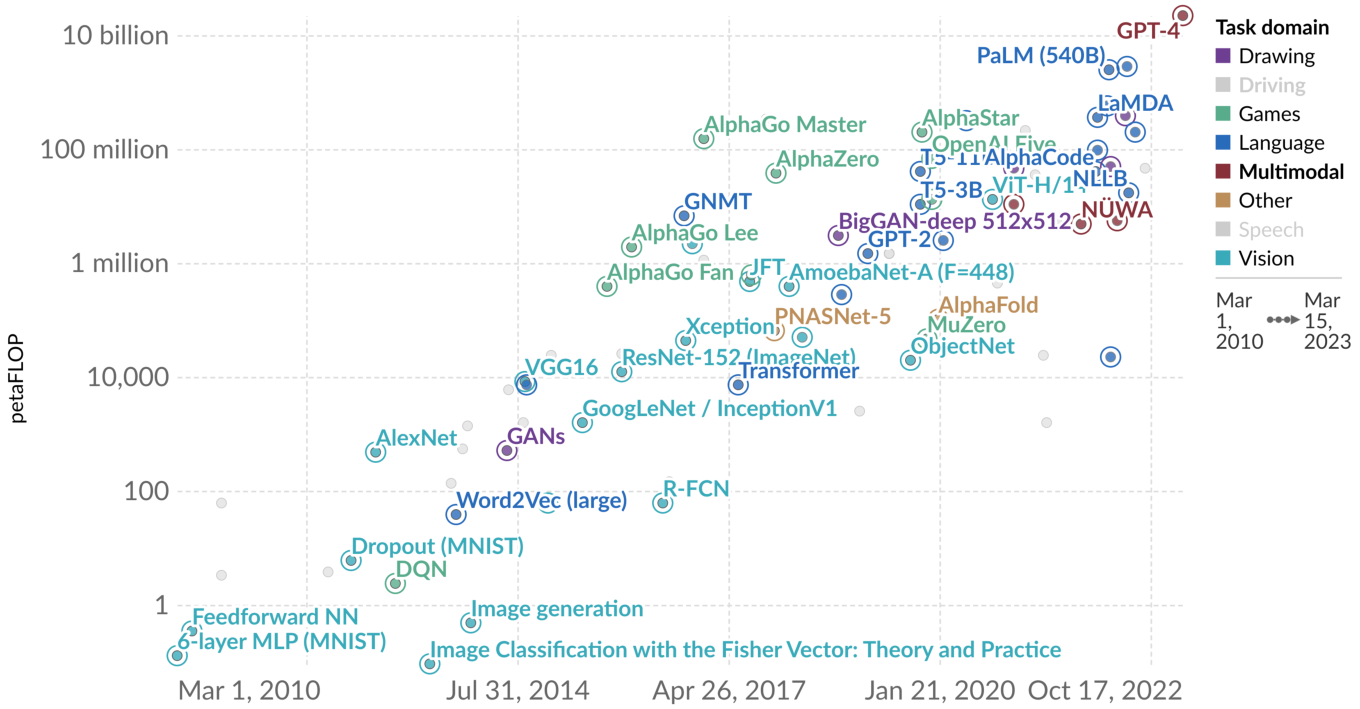
\includegraphics[width=0.9\textwidth]{../images/Compute_Budget_Training_Milestone_models_2022_mod.pdf}}

\vspace{-0.5cm}

\footnote<.->{\tiny Sevilla et al., 2023;
  OurWorldInData.org/artificial-intelligence; CC BY Source}

\end{frame}

\begin{frame}{Deep Learning \& Distributed Training}
\protect\hypertarget{deep-learning-distributed-training-1}{}

\begin{itemize}
\tightlist
\item
  Compute demand increases exponentially, 3.4 months doubling time since
  2012
\end{itemize}

\vspace{-0.1cm}
\center{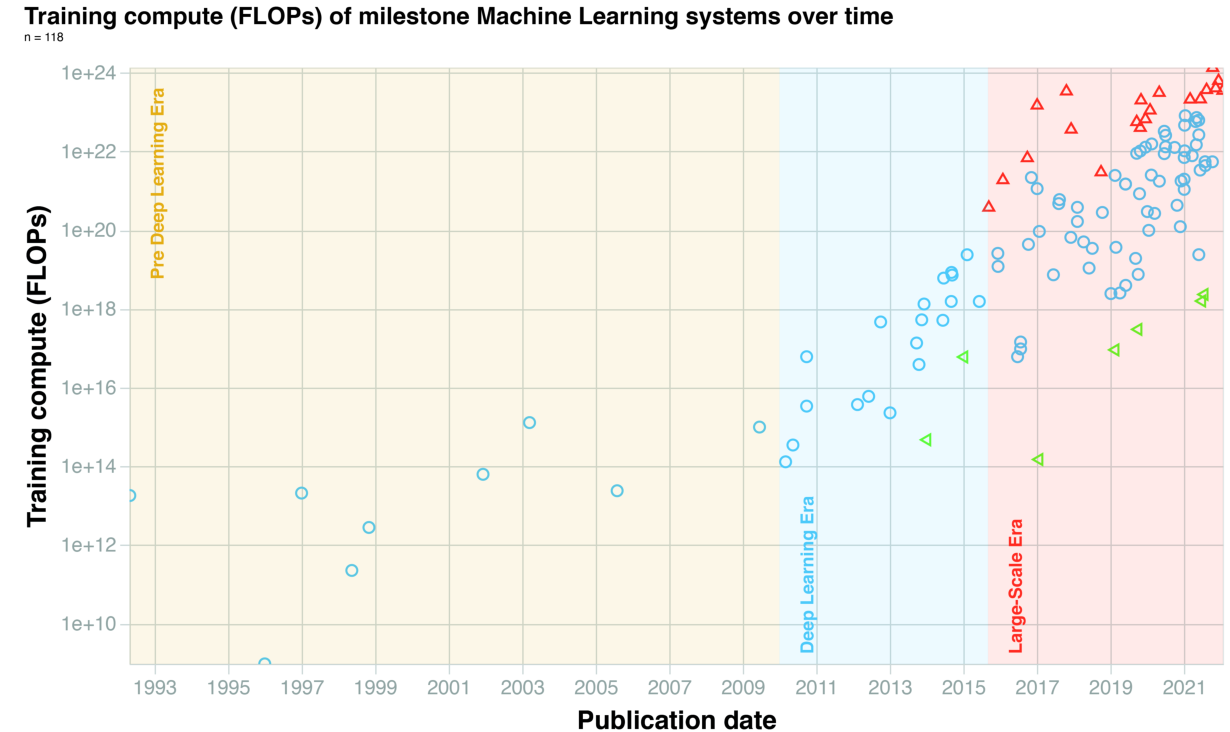
\includegraphics[width=0.8\textwidth]{../images/Compute_Budget_Eras_FLOPS_2022_mod.pdf}}

\footnote<.->{\tiny Sevilla et al., arXiv:2202.05924, 2023}

\end{frame}

\begin{frame}{Deep Learning \& Distributed Training}
\protect\hypertarget{deep-learning-distributed-training-2}{}

\begin{itemize}
\tightlist
\item
  Networks : large models, many layers, large number of parameters
  (weights)

  \begin{itemize}
  \tightlist
  \item
    Vision: Convolutional, Transformer and Hybrid networks
  \item
    hundreds of layers, hundred millions of parameters (currently up to
    20B)
  \end{itemize}
\end{itemize}

\center{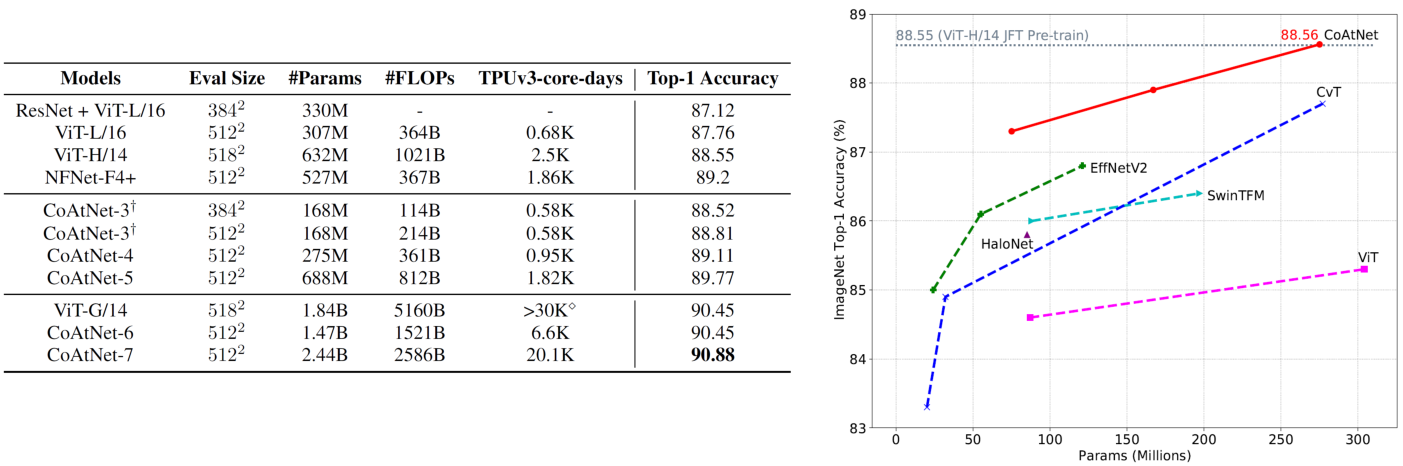
\includegraphics[width=\textwidth]{../images/Vision_Networks_CoAtNet_2021_mod.pdf}}

\footnote<.->{\tiny Dai et al, NeurIPS, 2021}

\end{frame}

\begin{frame}{Deep Learning \& Distributed Training}
\protect\hypertarget{deep-learning-distributed-training-3}{}

\begin{itemize}
\tightlist
\item
  Networks : large models, many layers, large number of parameters
  (weights)

  \begin{itemize}
  \tightlist
  \item
    Language: Transformer networks
  \item
    hundreds of layers, billions of parameters (GPT-3: 175 Billion)
  \end{itemize}
\end{itemize}

\center{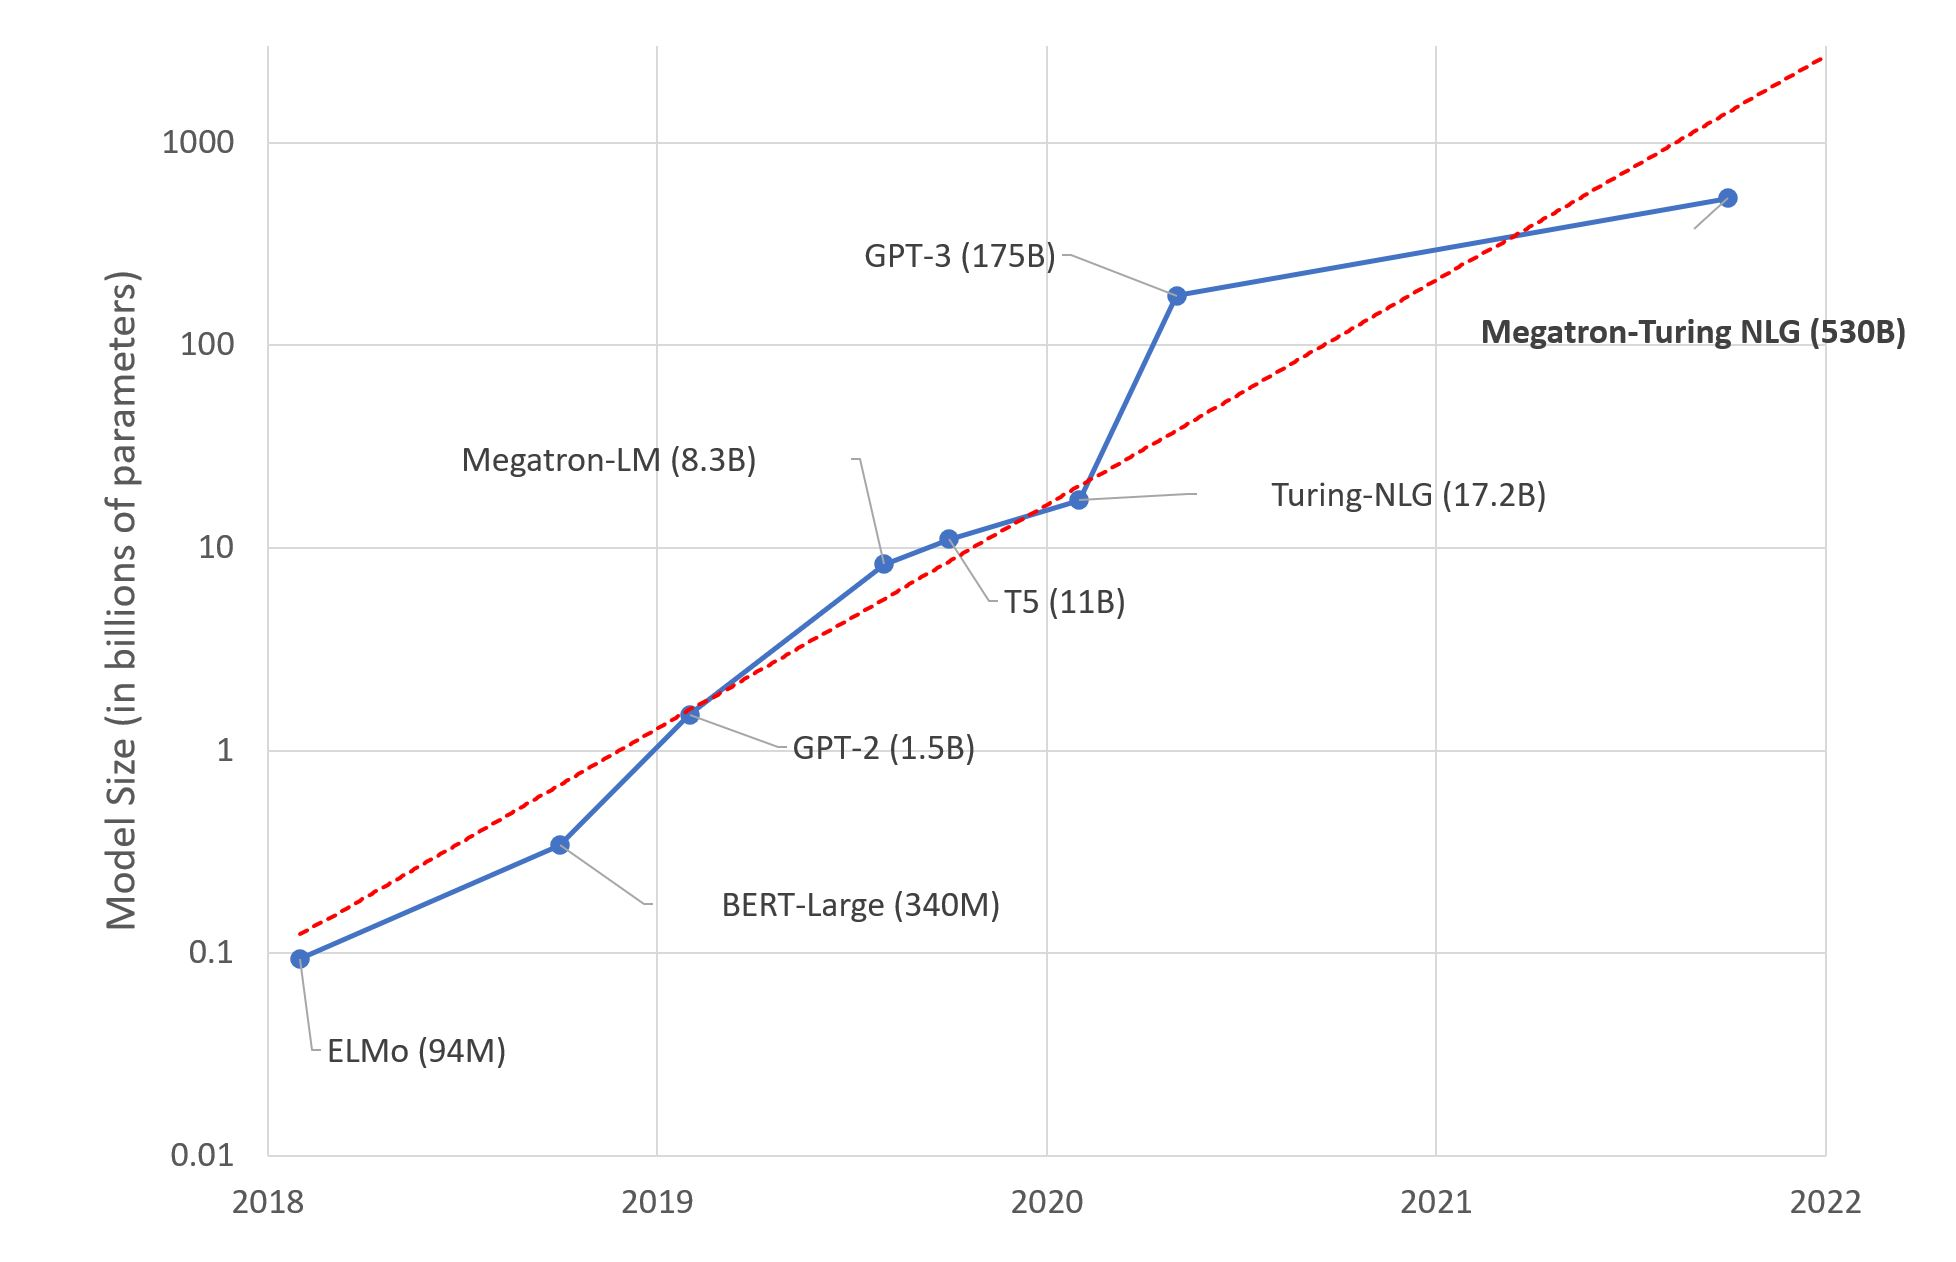
\includegraphics[width=0.65\textwidth]{../images/MegaTron_DeepSpeed_Microsoft_Turing_NLM_model-size-graph.jpg}}

\vspace*{-1cm}

\footnote<.->{\tiny Narayanan et al, 2021}

\end{frame}

\begin{frame}{Deep Learning \& Distributed Training}
\protect\hypertarget{deep-learning-distributed-training-4}{}

\begin{itemize}
\tightlist
\item
  GPT-3: 175 billions weights, \(\approx\) 350 GB, does not fit on
  single GPU (A100: 40/80GB)
\item
  ResNets, ViT \(<\) 1B weights, \(\lesssim\) 40 GB, fit on single GPU

  \begin{itemize}
  \tightlist
  \item
    depending on chosen resolution of input \(X\) and batch size
    \(\vert B \vert\)!
  \end{itemize}
\end{itemize}

\center{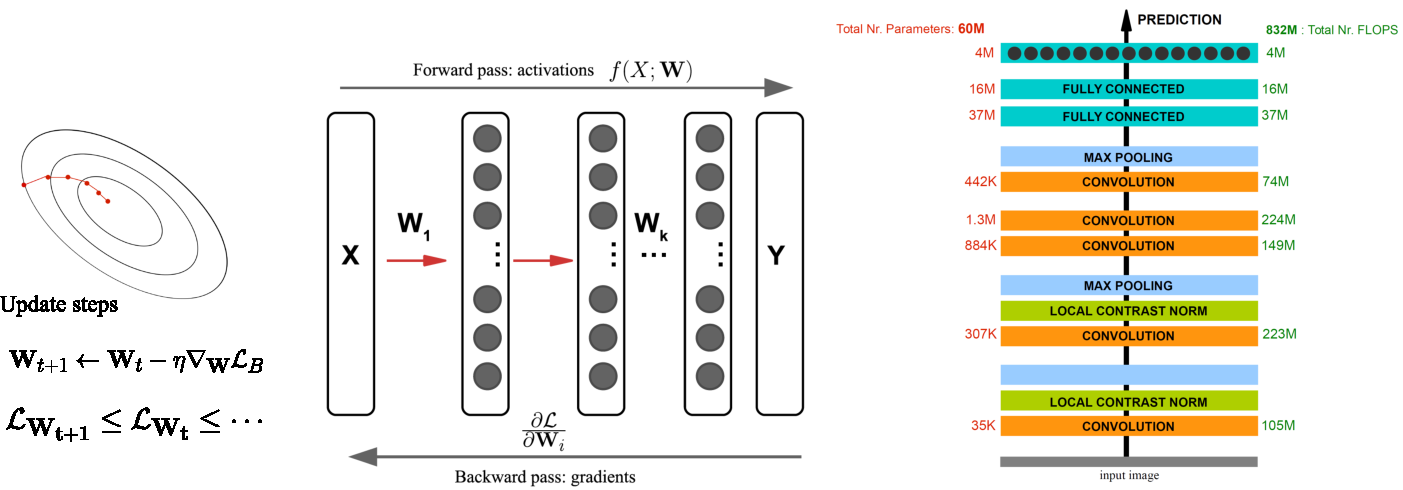
\includegraphics[width=\textwidth]{../images/Network_Computation_Size_AlexNet.pdf}}

\end{frame}

\begin{frame}{Deep Learning \& Distributed Training}
\protect\hypertarget{deep-learning-distributed-training-5}{}

\begin{itemize}
\tightlist
\item
  GPT-3: 175 billions weights, \(\approx\) 350 GB, does not fit on
  single GPU
\item
  ResNets, ViT \(<\) 1B weights, \(\lesssim\) 40 GB, fit on single GPU

  \begin{itemize}
  \tightlist
  \item
    depending on chosen resolution of input \(X\) and batch size
    \(\vert B \vert\)!
  \end{itemize}
\end{itemize}

\center{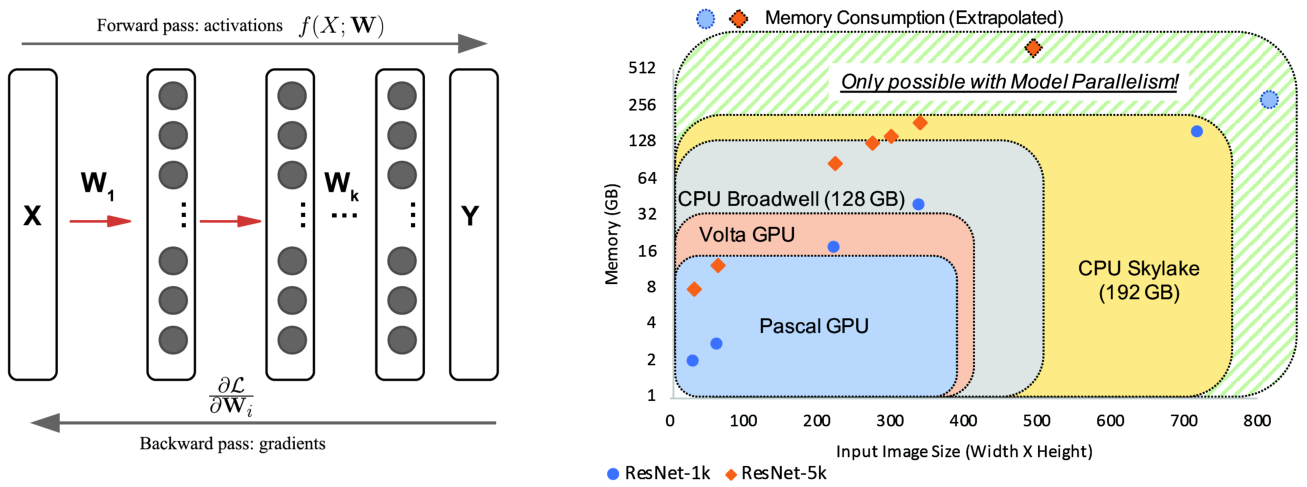
\includegraphics[width=0.9\textwidth]{../images/Only_Possible_with_X_Parallelism.pdf}}

\footnote<.->{\tiny Awan et al., 2020}

\end{frame}

\begin{frame}{Distributed Training}
\protect\hypertarget{distributed-training}{}

\begin{itemize}
\tightlist
\item
  Use the computational power and memory capacity of multiple nodes of a
  large machine
\item
  Requires taking care of internode communication
\end{itemize}

\center{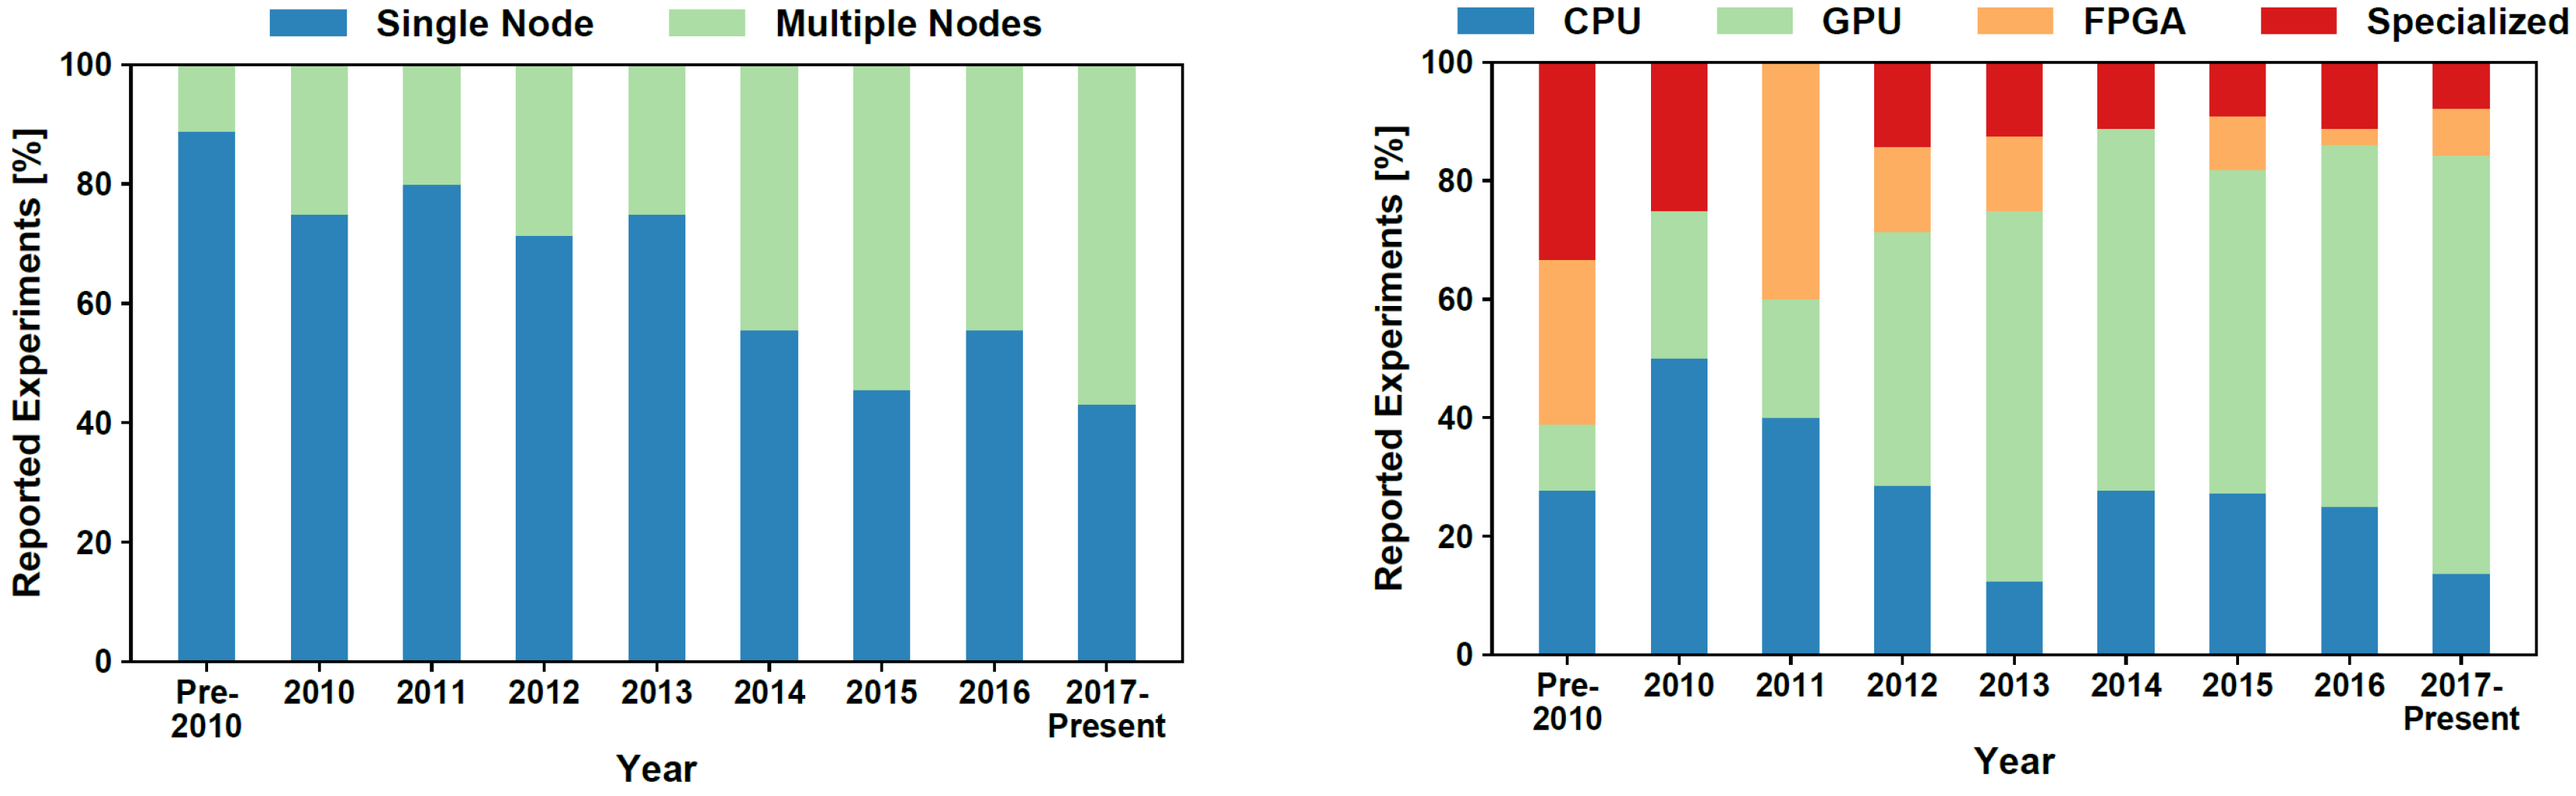
\includegraphics[width=0.9\textwidth]{../images/MultiNode_Training_Accellerators.png}}

\footnote<.->{\tiny Ben-Nun \& Hoefler, 2018}

\end{frame}

\begin{frame}{Distributed Training}
\protect\hypertarget{distributed-training-1}{}

\begin{itemize}
\tightlist
\item
  Use the computational power and memory capacity of multiple nodes of a
  large machine
\item
  Requires taking care of internode communication
\item
  Requires high bandwidth interconnect between the compute nodes

  \begin{itemize}
  \tightlist
  \item
    HPC: InfiniBand (4x Mellanox 200 Gb/s cards on JUWELS Booster per
    node)
  \item
    Not available on conventional clusters!
  \end{itemize}
\end{itemize}

\center{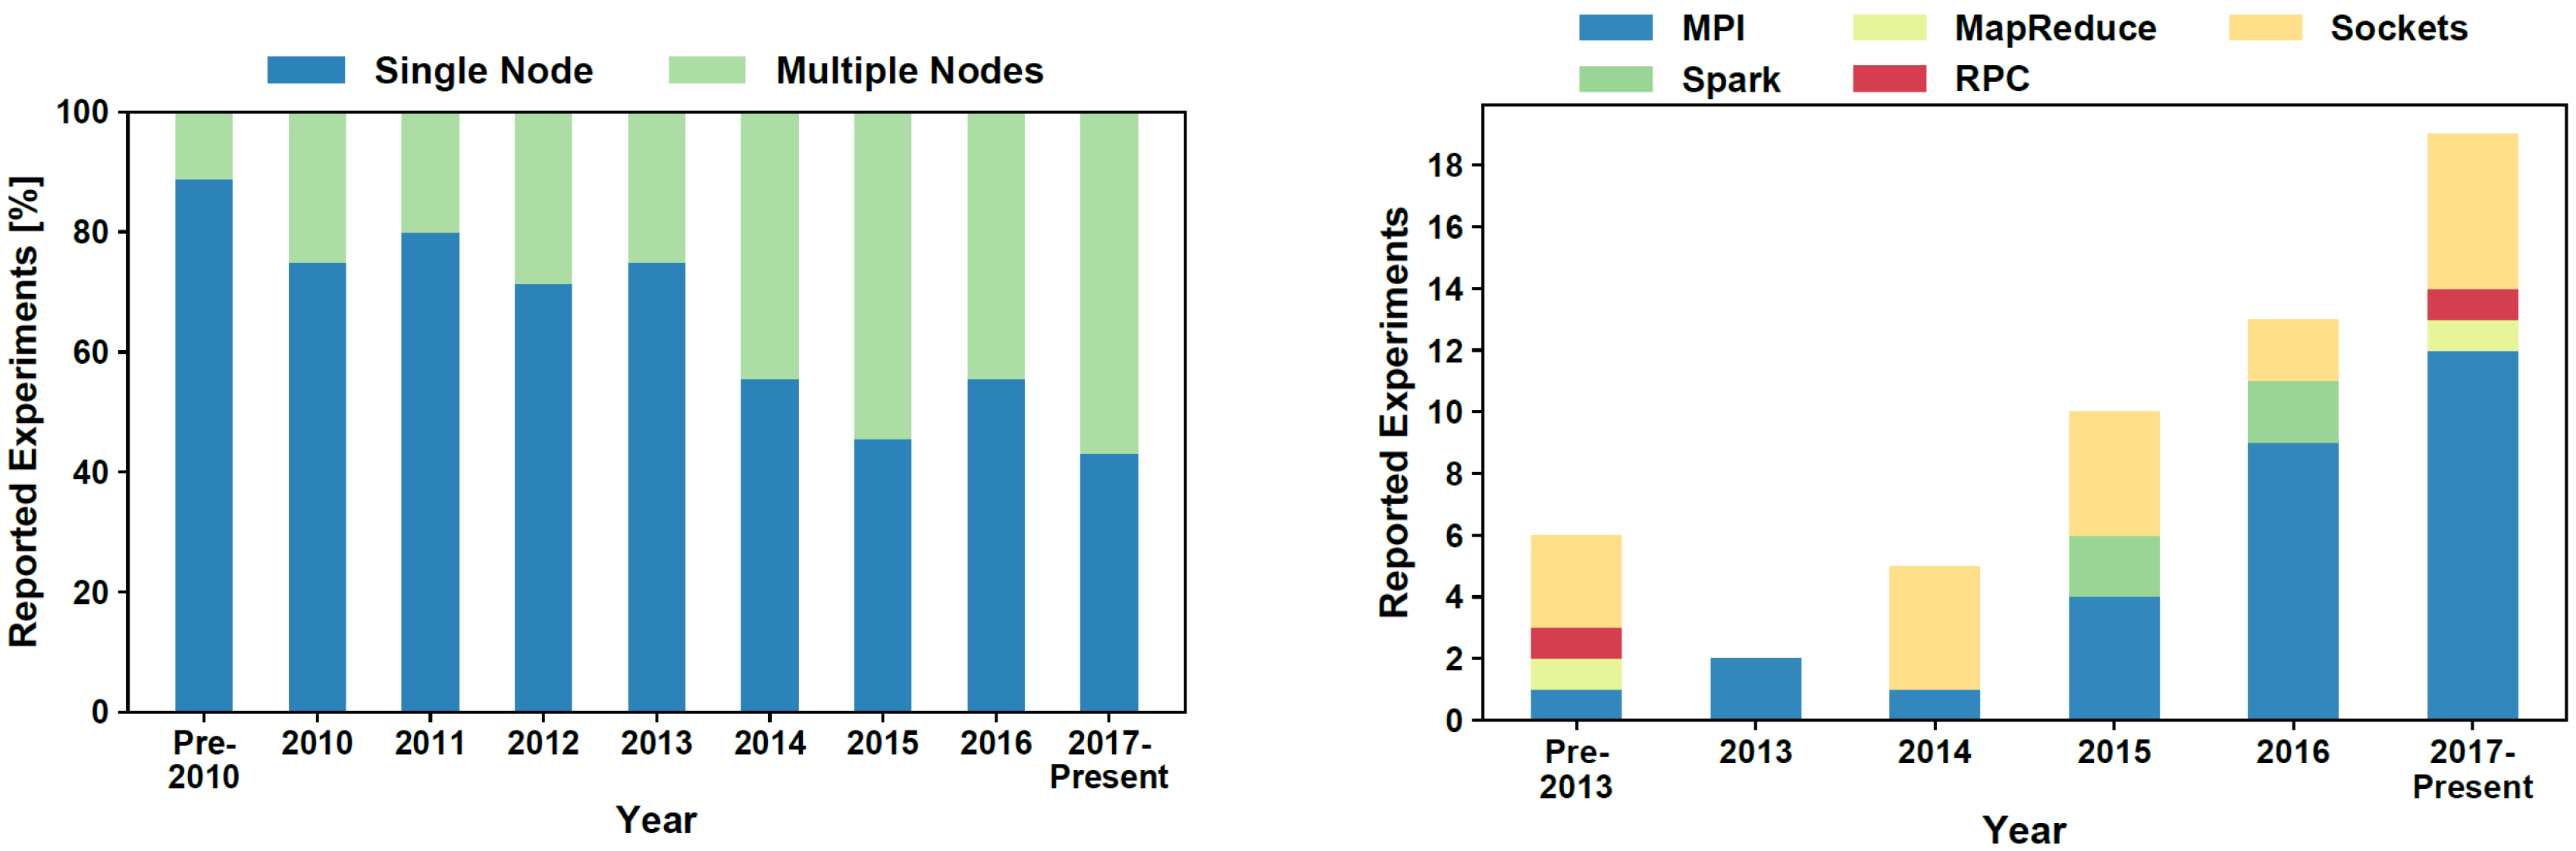
\includegraphics[width=0.9\textwidth]{../images/MultiNode_Training_Communication_Collectives.png}}

\footnote<.->{\tiny Ben-Nun \& Hoefler, 2018}

\end{frame}

\begin{frame}{Distributed Training}
\protect\hypertarget{distributed-training-2}{}

\begin{itemize}
\tightlist
\item
  Depending on whether full model fits on a single GPU, different
  schemes

  \begin{itemize}
  \tightlist
  \item
    data parallelism: split only data across GPUs, model cloned on each
    GPU
  \item
    model parallelism: split within layers across GPUs
  \item
    pipeline parallelism: split layer groups across GPUs
  \end{itemize}
\end{itemize}

\center{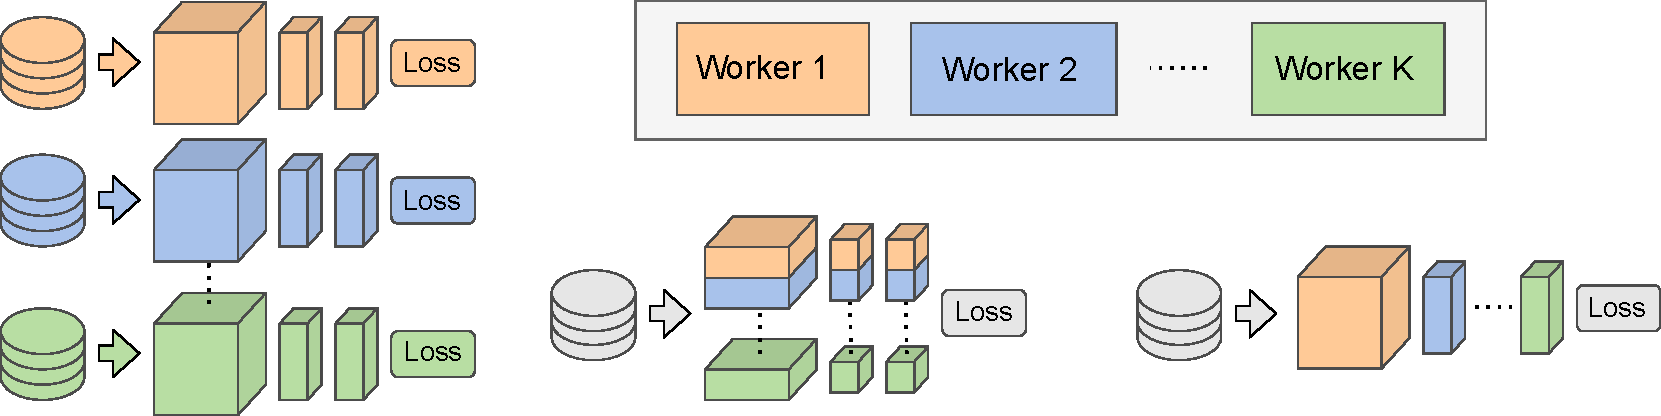
\includegraphics[width=\textwidth]{../images/Distributed_Training_Schemes_Workers.pdf}}

\footnote<.->{\tiny Laskin et al., 2020}

\end{frame}

\begin{frame}{Distributed Training}
\protect\hypertarget{distributed-training-3}{}

\begin{itemize}
\tightlist
\item
  Model does not fit on single GPU: no training without parallelization
  possible at all

  \begin{itemize}
  \tightlist
  \item
    AlexNet in 2012; GPT-3; CLIP ViT G/14, \ldots{}
  \end{itemize}
\item
  Model fits on single GPU: why distributed training?

  \begin{itemize}
  \tightlist
  \item
    multiple GPUs can drastically speed up training phase
    --\textgreater{} \textbf{data parallelism}

    \begin{itemize}
    \tightlist
    \item
      e.g.~ImageNet training: from days to hours or minutes
    \end{itemize}
  \end{itemize}
\end{itemize}

\center{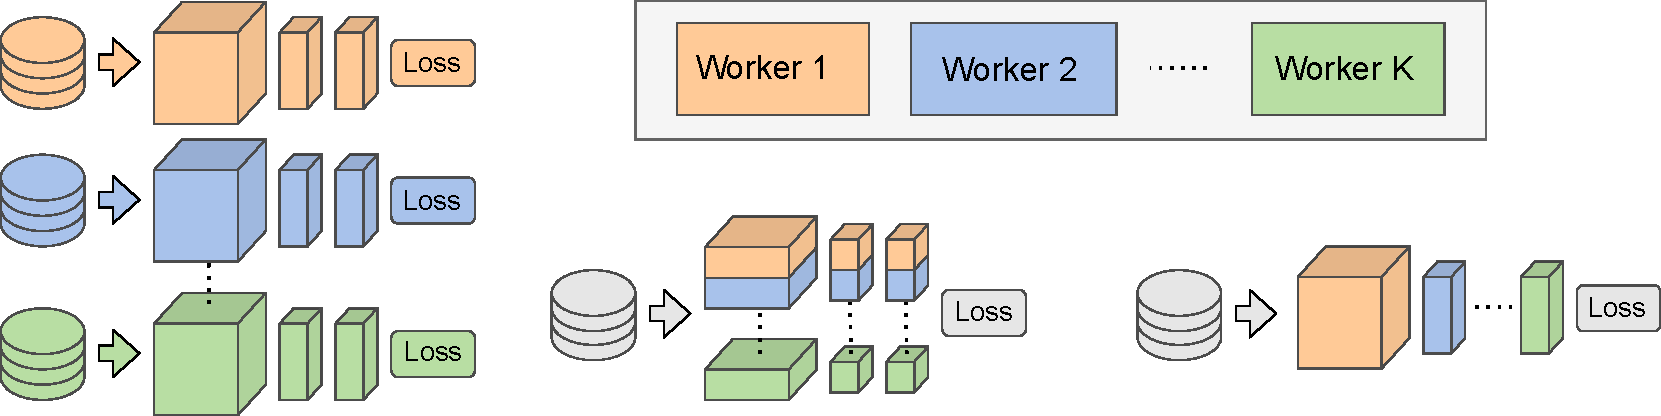
\includegraphics[width=\textwidth]{../images/Distributed_Training_Schemes_Workers.pdf}}

\footnote<.->{\tiny Laskin et al., 2020}

\end{frame}

\begin{frame}{Distributed Training}
\protect\hypertarget{distributed-training-4}{}

\begin{itemize}
\tightlist
\item
  ImageNet distributed training: from days, to hours, to minutes
\end{itemize}

\center{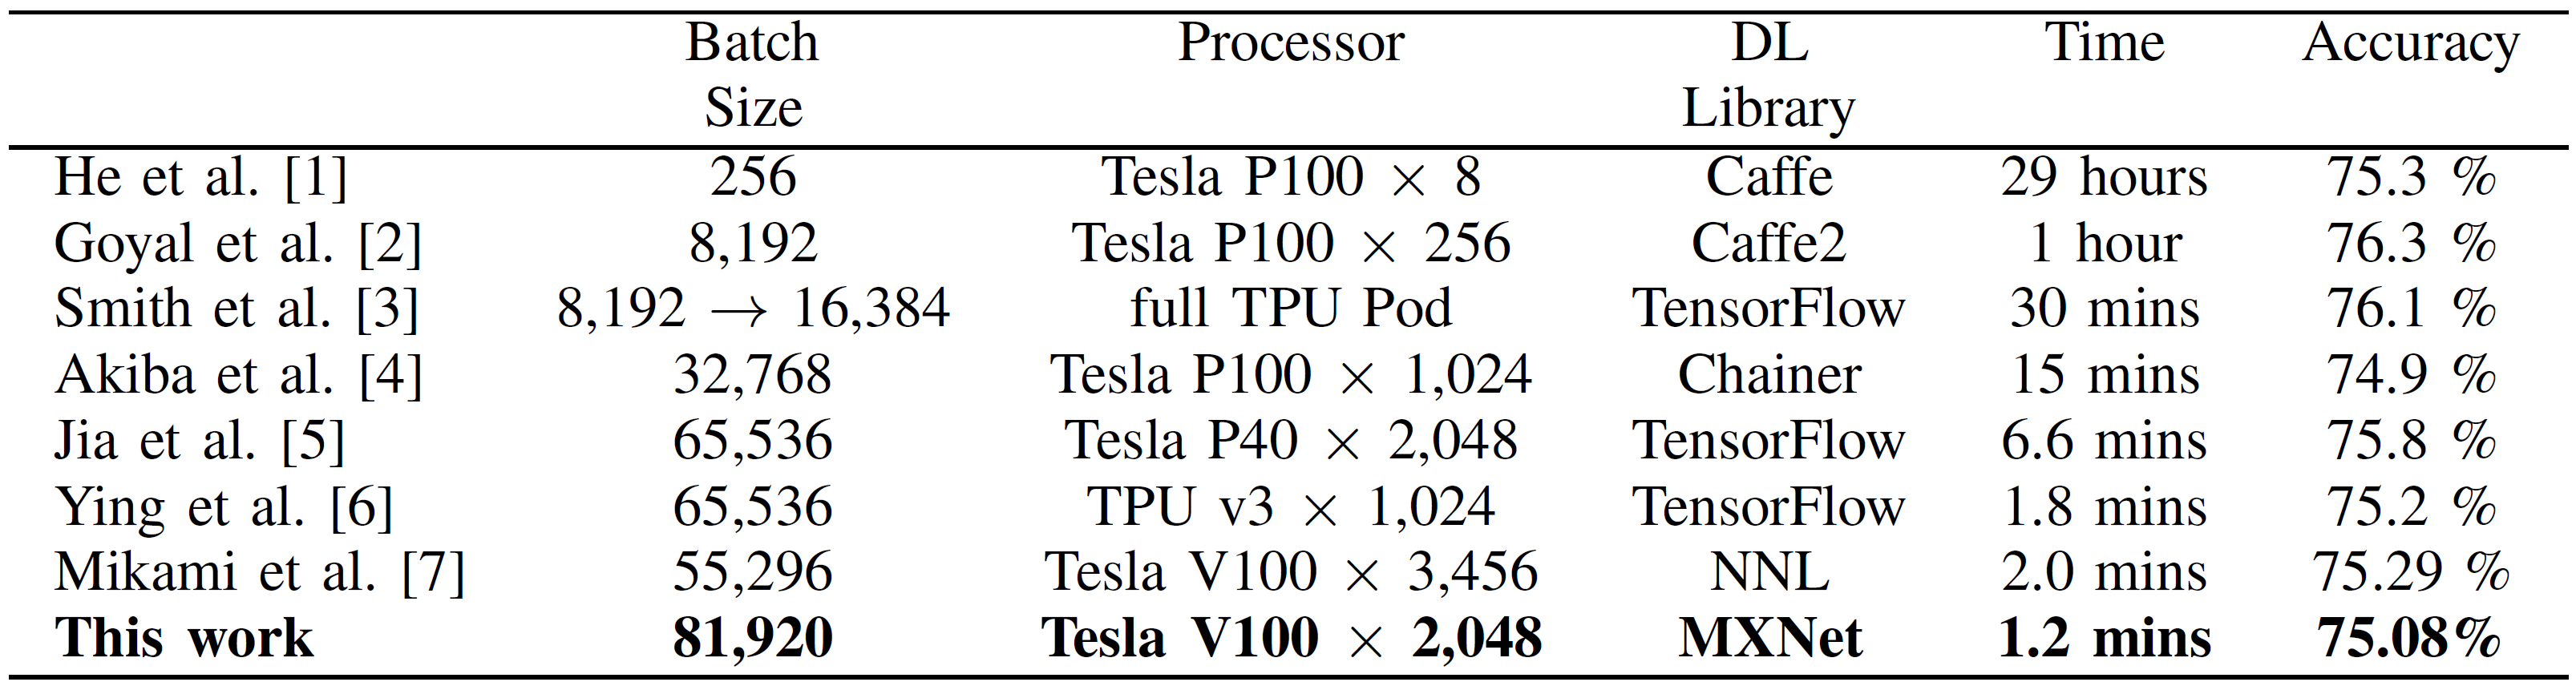
\includegraphics[width=0.7\textwidth]{../images/Yamazaki_RunTime_Table_ImageNet_ResNet-50_Accuracies.png}}

\center{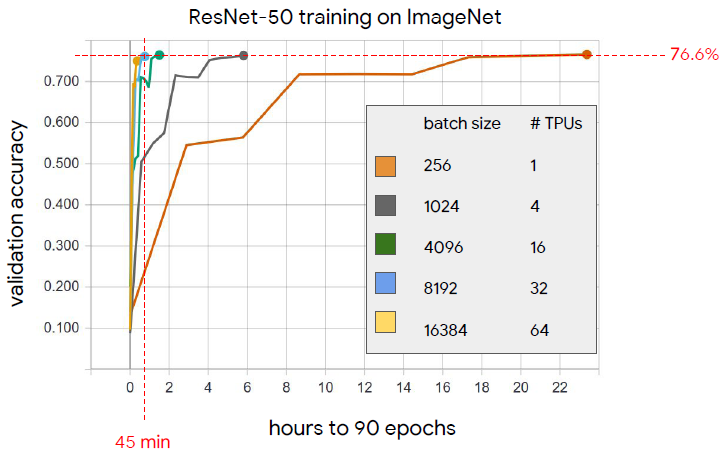
\includegraphics[width=0.45\textwidth]{../images/ResNet-50_ImageNet_Training_Time_Validation_Accuracy}}

\vspace*{-1cm}

\footnote<.->{\tiny Yamazoto et al., 2019; Ying, 2018}

\end{frame}

\begin{frame}{Deep Learning with Data Parallelism}
\protect\hypertarget{deep-learning-with-data-parallelism}{}

\begin{itemize}
\tightlist
\item
  Data parallelism: simple approach for efficient distributed training

  \begin{itemize}
  \tightlist
  \item
    whole network model \textbf{has to} fit on one GPU: depends on batch
    size!
  \item
    split whole dataset across multiple workers
  \item
    speeds up model training -- given good scaling and well-tuned
    learning
  \end{itemize}
\item
  Faster training, shorter experiment cycle -- more opportunities to
  test new ideas and models
\end{itemize}

\center{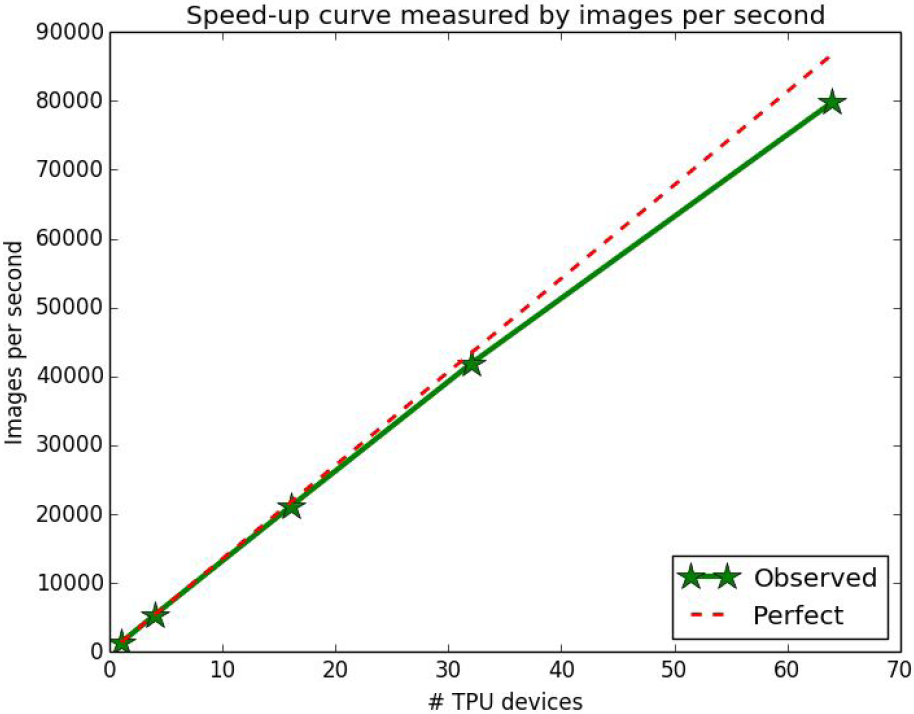
\includegraphics[width=0.4\textwidth]{../images/ImageNet-1k_TPUs_Ims.png}}

\footnote<.->{\tiny Ying, 2018}

\end{frame}

\begin{frame}{Deep Learning with Data Parallelism}
\protect\hypertarget{deep-learning-with-data-parallelism-1}{}

\begin{itemize}
\tightlist
\item
  Data parallelism: simple approach for efficient distributed training

  \begin{itemize}
  \tightlist
  \item
    whole network model \textbf{has to} fit on one GPU: depends on batch
    size!
  \item
    split whole dataset across multiple workers
  \item
    good scaling: necessary (but not sufficient!) for model training
    speed up
  \end{itemize}
\item
  Faster training, shorter experiment cycle -- more opportunities to
  test new ideas and models
\end{itemize}

\center{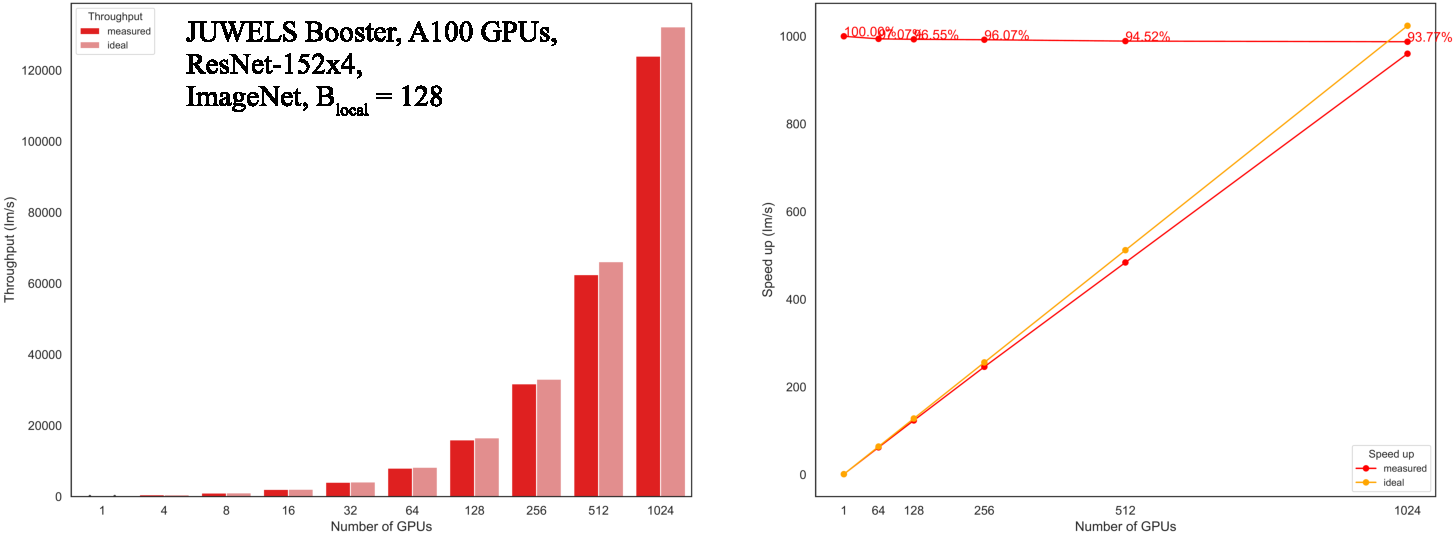
\includegraphics[width=0.9\textwidth]{../images/JUWELS_Booster_Ims_SpeedUp_ResNet-152x4_mod.pdf}}

\footnote<.->{\tiny Cherti and Jitsev, arXiv:2106.00116, MedNeurIPS
  Workshop, 2021}

\end{frame}

\begin{frame}{Deep Learning with Data Parallelism}
\protect\hypertarget{deep-learning-with-data-parallelism-2}{}

\begin{itemize}
\tightlist
\item
  Data parallelism: simple approach for efficient distributed model
  training

  \begin{itemize}
  \tightlist
  \item
    same model is cloned across \(K\) workers
  \item
    each model clone trains on its dedicated subset of total available
    data
  \item
    synchronous (S-SGD) or asynchronous (A-SGD) optimization; central
    (parameter server) or decentralized (ring-AllReduce) communication
    for weight updates
  \end{itemize}
\end{itemize}

\center{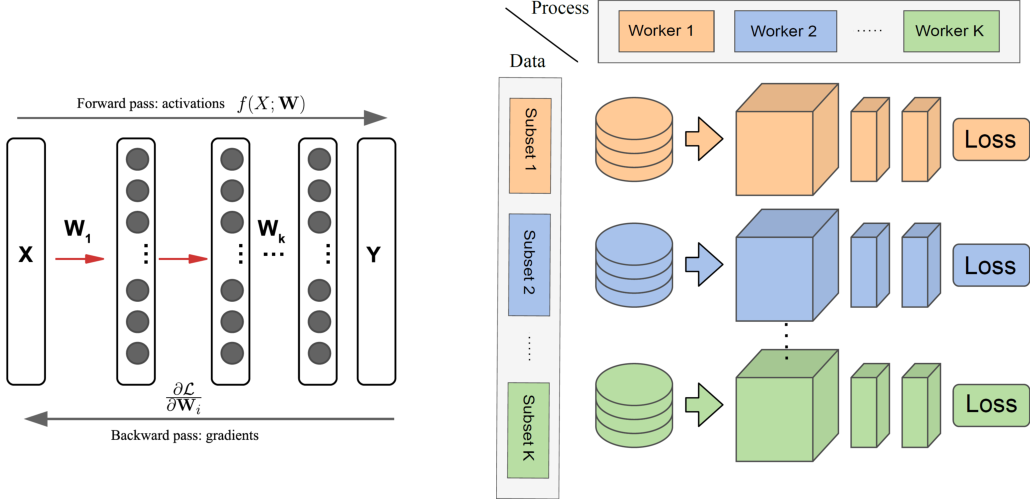
\includegraphics[width=0.8\textwidth]{../images/Data_Parallel_Scheme_Model_Workers_Processes_Data.pdf}}

\end{frame}

\begin{frame}{Deep Learning with Data Parallelism}
\protect\hypertarget{deep-learning-with-data-parallelism-3}{}

\begin{itemize}
\tightlist
\item
  Data parallelism: simple approch for efficient distributed model
  training

  \begin{itemize}
  \tightlist
  \item
    can be understood as training a model using a larger mini-batch size
    \(\vert \mathfrak{B} \vert\)

    \begin{itemize}
    \tightlist
    \item
      \(\mathfrak{B} = B_1 \cup \ldots \cup B_K\),
      \(B_i \cap B_j = \emptyset,\ \forall i,j \in K\) workers
      \vspace*{2mm}
    \item
      \(\vert \mathfrak{B} \vert = K \cdot \vert B_{\text{ref}} \vert\),
      where \(\vert B_{\text{ref}} \vert = n\) is original, reference
      batch size for a single worker
    \end{itemize}
  \end{itemize}
\end{itemize}

\center{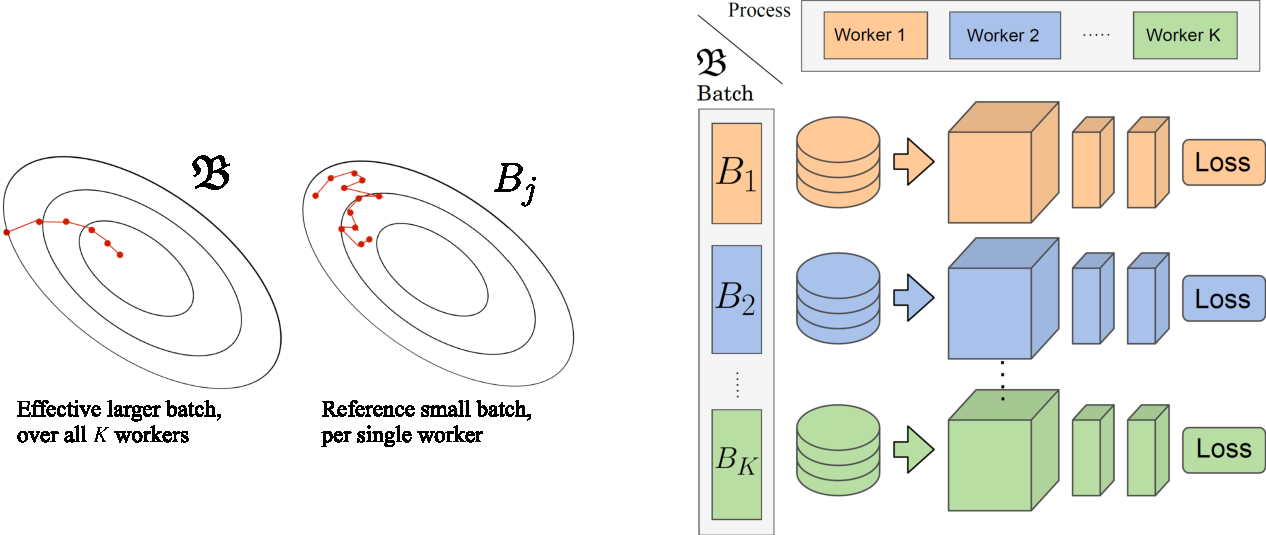
\includegraphics[width=0.8\textwidth]{../images/Large_Small_Reference_Batch_Data_Parallel_Model_Workers_Processes.pdf}}

\end{frame}

\begin{frame}{Reminder: Mini-Batch SGD}
\protect\hypertarget{reminder-mini-batch-sgd}{}

\begin{itemize}
\tightlist
\item
  Mini-batch SGD

  \begin{itemize}
  \item
    perform an update step using loss gradient
    \(\nabla_\mathbf{W} \mathcal{L}_B\) over a \textbf{mini-batch} of
    size \(\vert B \vert = n \ll N\)
    \[ \nabla_\mathbf{W} \mathcal{L}_B = \nabla_\mathbf{W} \dfrac{1}{n} {\displaystyle \sum_{X_i \in B} \mathcal{L}_i} \]
  \item
    update step:
    \(\mathbf{W}_{t+1} \leftarrow \mathbf{W}_t - \eta \nabla_\mathbf{W} \mathcal{L}_B\)
  \end{itemize}
\end{itemize}

\center{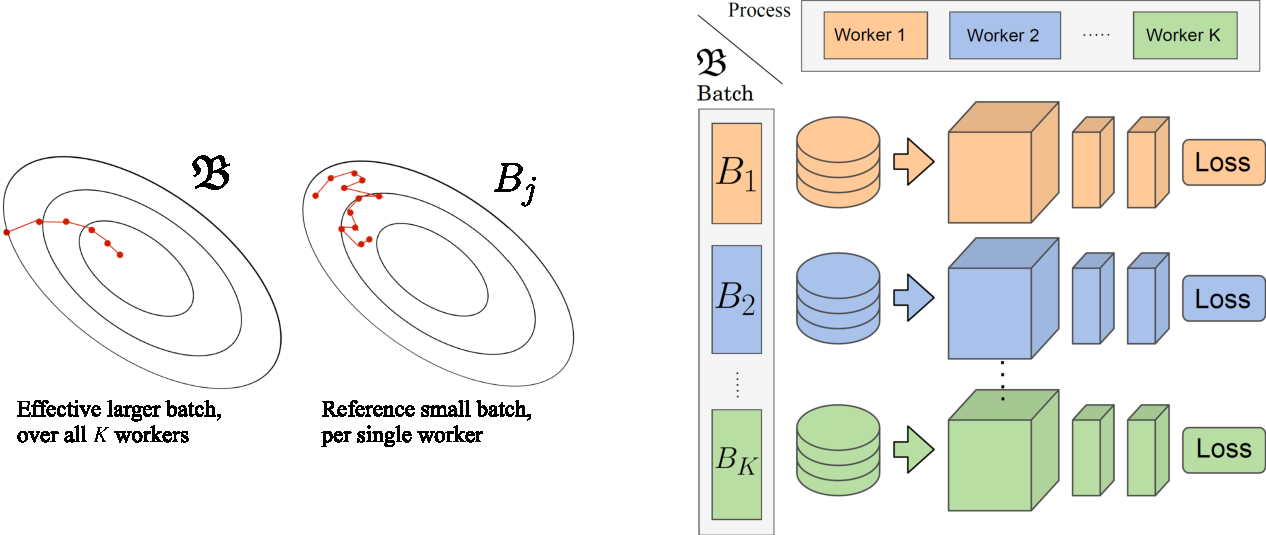
\includegraphics[width=0.8\textwidth]{../images/Large_Small_Reference_Batch_Data_Parallel_Model_Workers_Processes.pdf}}

\end{frame}

\begin{frame}{Deep Learning with Data Parallelism}
\protect\hypertarget{deep-learning-with-data-parallelism-4}{}

\begin{itemize}
\tightlist
\item
  \textbf{Effective larger mini-batch} \(\mathfrak{B}\) over \(K\)
  workers

  \begin{itemize}
  \tightlist
  \item
    perform an update step using loss gradient
    \(\nabla_\mathbf{W} \mathcal{L}_{\mathfrak{B}}\) over a larger
    \textbf{effective} mini-batch
    \(\vert \mathfrak{B} \vert = K \cdot \vert B_{\text{ref}}\vert,\ \vert B \vert = n \ll N\)
    \[ \nabla_\mathbf{W} \mathcal{L}_{\mathfrak{B}} = \nabla_\mathbf{W} \dfrac{1}{K} {\displaystyle \sum_{j = 1}^{K} } \dfrac{1}{n} {\displaystyle \sum_{X_i \in B_j} \mathcal{L}_i} = \nabla_\mathbf{W} \dfrac{1}{nK} {\displaystyle \sum_{X_i \in \mathfrak{B}} \mathcal{L}_i} \]
  \item
    update step:
    \(\mathbf{W}_{t+1} \leftarrow \mathbf{W}_t - \eta \nabla_\mathbf{W} \mathcal{L}_{\mathfrak{B}}\)
  \end{itemize}
\end{itemize}

\center{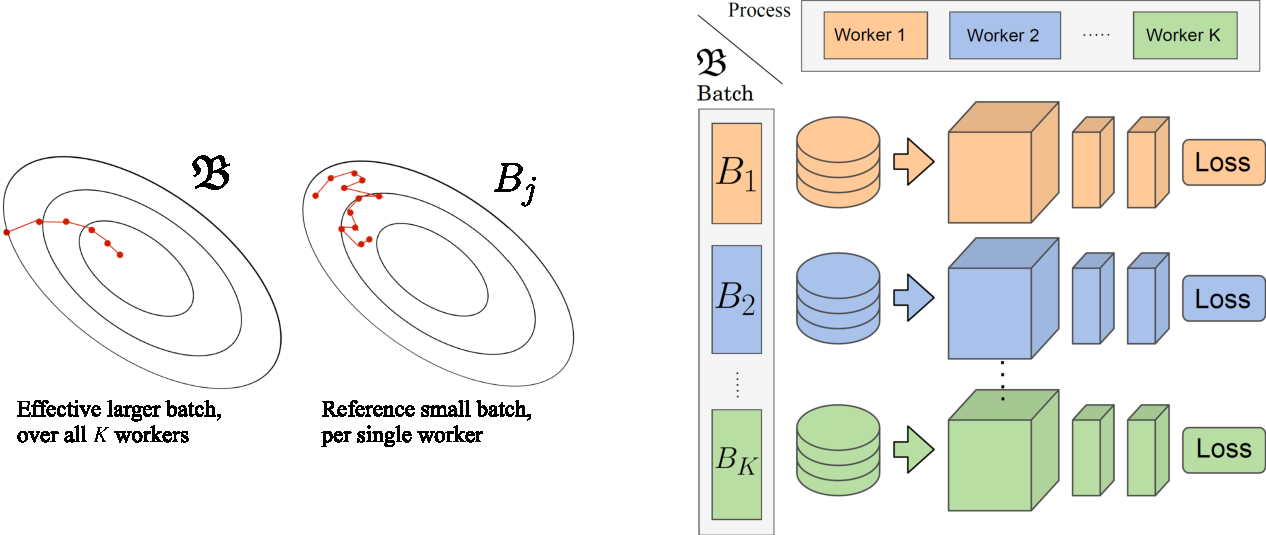
\includegraphics[width=0.8\textwidth]{../images/Large_Small_Reference_Batch_Data_Parallel_Model_Workers_Processes.pdf}}

\end{frame}

\begin{frame}{Deep Learning with Data Parallelism}
\protect\hypertarget{deep-learning-with-data-parallelism-5}{}

\begin{itemize}
\tightlist
\item
  Training a model using a larger mini-batch size
  \(\vert \mathfrak{B} \vert\)

  \begin{itemize}
  \tightlist
  \item
    \(\vert \mathfrak{B} \vert = K \cdot \vert B_{\text{ref}} \vert\),
    where \(\vert B_{\text{ref}} \vert\) is original, reference batch
    size for a single worker
  \item
    Update step:
    \(\mathbf{W}_{t+1} \leftarrow \mathbf{W}_t - \eta \nabla_\mathbf{W} \mathcal{L}_{\mathfrak{B}}\)
  \item
    \textbf{Reminder:} Changes optimization trajectory and weight
    dynamics compared to smaller mini-batch training
  \end{itemize}
\end{itemize}

\center{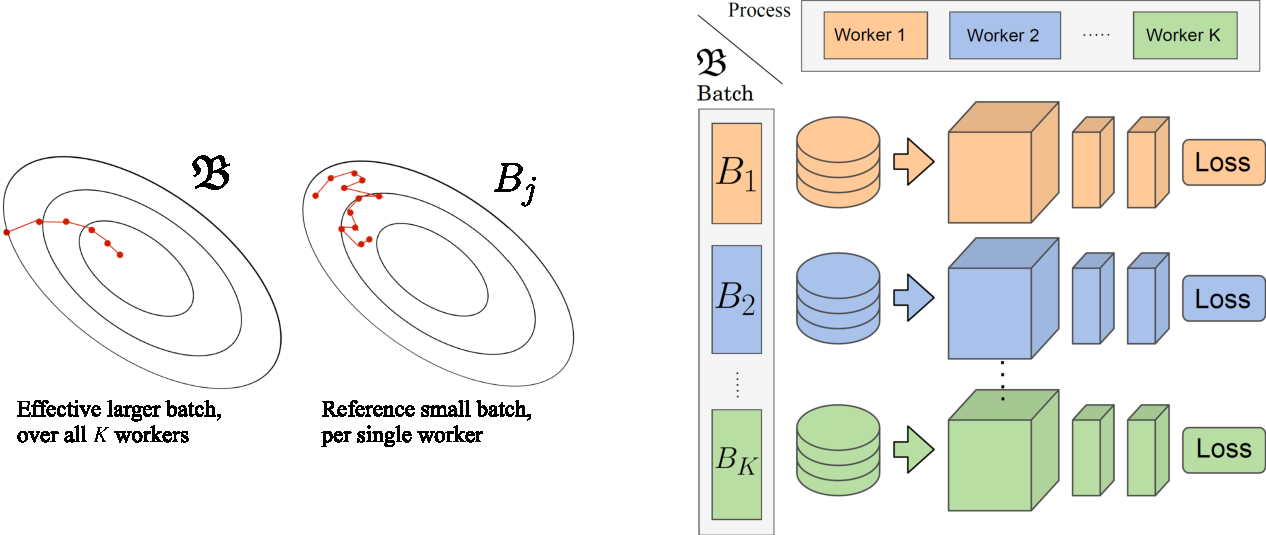
\includegraphics[width=0.8\textwidth]{../images/Large_Small_Reference_Batch_Data_Parallel_Model_Workers_Processes.pdf}}

\end{frame}

\begin{frame}{Deep Learning with Data Parallelism}
\protect\hypertarget{deep-learning-with-data-parallelism-6}{}

\begin{itemize}
\tightlist
\item
  Training a model using a larger mini-batch size
  \(\vert \mathfrak{B} \vert\)

  \begin{itemize}
  \tightlist
  \item
    \(\vert \mathfrak{B} \vert = K \cdot \vert B_{\text{ref}} \vert\),
    where \(\vert B_{\text{ref}} \vert\) is original, reference batch
    size for a single worker
  \item
    Update step:
    \(\mathbf{W}_{t+1} \leftarrow \mathbf{W}_t - \eta \nabla_\mathbf{W} \mathcal{L}_{\mathfrak{B}}\)
  \item
    \textbf{Reminder:} Changes optimization trajectory and weight
    dynamics compared to smaller mini-batch training
  \end{itemize}
\end{itemize}

\center{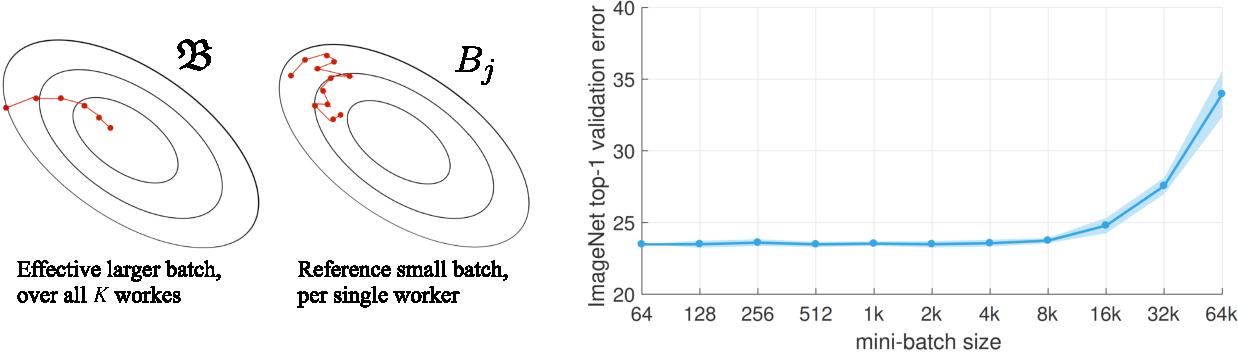
\includegraphics[width=0.8\textwidth]{../images/Effective_Reference_Batch_ImageNet_Goyal_2.pdf}}

\footnote<.->{\tiny Goyal et al., 2017}

\end{frame}

\begin{frame}{Deep Learning with Data Parallelism}
\protect\hypertarget{deep-learning-with-data-parallelism-7}{}

\begin{itemize}
\tightlist
\item
  Data parallel distributed training requires:

  \begin{itemize}
  \tightlist
  \item
    \textbf{proper data feeding} for each worker
  \item
    setting up workers, one per each GPU (model clones)
  \item
    \textbf{sync of model clone parameters} (weights) across workers:
    update step -- \textbf{communication load}

    \begin{itemize}
    \tightlist
    \item
      after each forward/backward pass on workers' mini-batches
    \item
      \(\nabla_\mathbf{W} \mathcal{L}_{\mathfrak{B}} = {\displaystyle \underbrace{\dfrac{1}{K} \sum_{j = 1}^{K}}_{\text{across } K \text{ workers}} } \underbrace{\nabla_\mathbf{W} \dfrac{1}{n} {\displaystyle \sum_{X_i \in B_j} \mathcal{L}_i}}_{\text{on worker } j}\)
    \end{itemize}
  \end{itemize}
\end{itemize}

\vspace*{-1.5cm}
\center{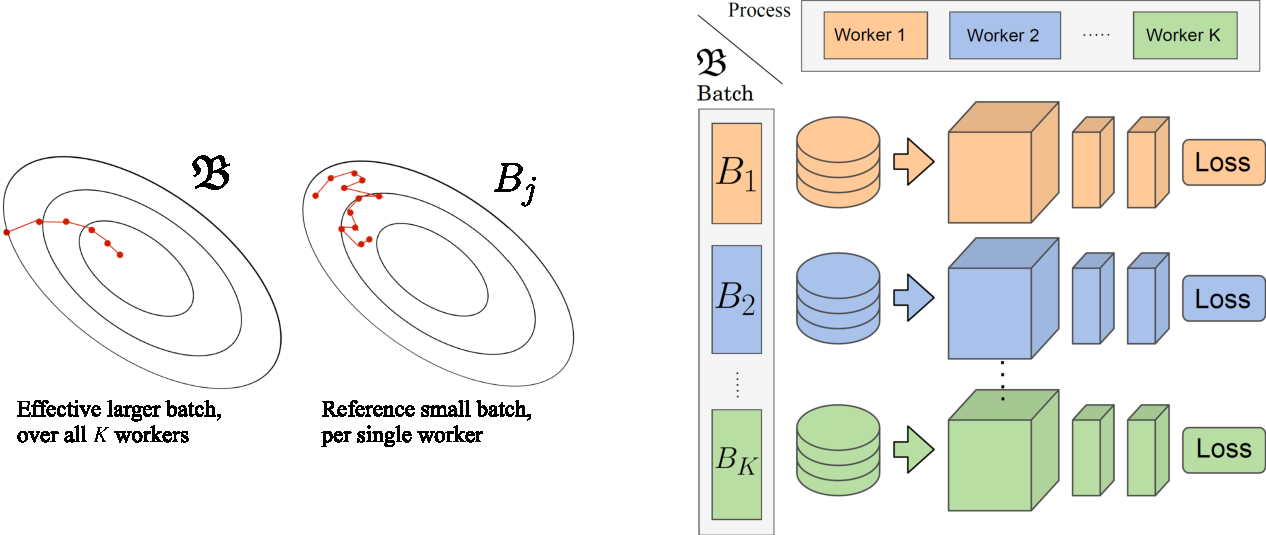
\includegraphics[width=0.8\textwidth]{../images/Large_Small_Reference_Batch_Data_Parallel_Model_Workers_Processes.pdf}}

\end{frame}

\begin{frame}{Deep Learning with Data Parallelism}
\protect\hypertarget{deep-learning-with-data-parallelism-8}{}

\begin{itemize}
\tightlist
\item
  Data parallelism: proper data feeding for each worker

  \begin{itemize}
  \tightlist
  \item
    important not to let GPUs ``starve'' while training
  \end{itemize}
\end{itemize}

\center{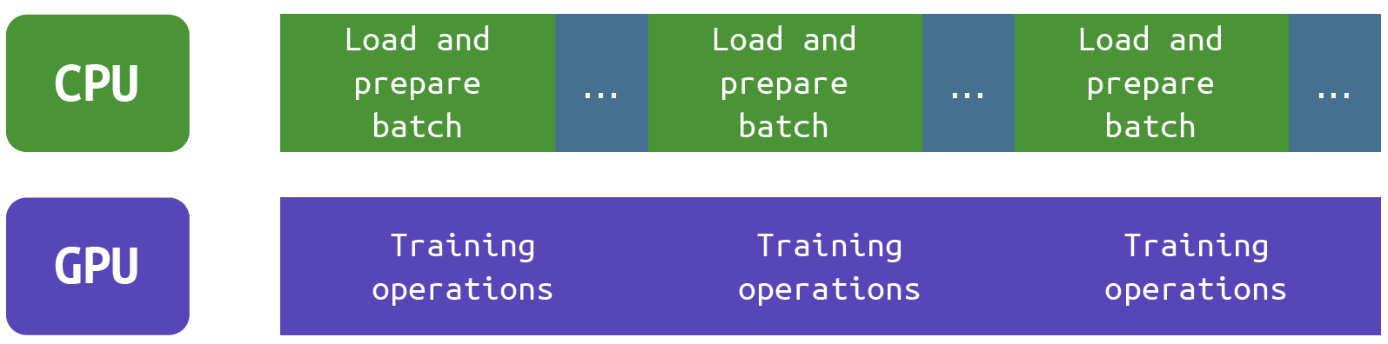
\includegraphics[width=0.9\textwidth]{../images/GPU_CPU_Data_Training_1.pdf}}

\footnote<.->{\tiny Figure: Mendonça, Sarmiento, ETH CSCS, 2020}

\end{frame}

\begin{frame}{Deep Learning with Data Parallelism}
\protect\hypertarget{deep-learning-with-data-parallelism-9}{}

\begin{itemize}
\tightlist
\item
  Data parallelism: proper data feeding for each worker

  \begin{itemize}
  \tightlist
  \item
    important not to let GPUs ``starve'' while training
  \end{itemize}
\end{itemize}

\center{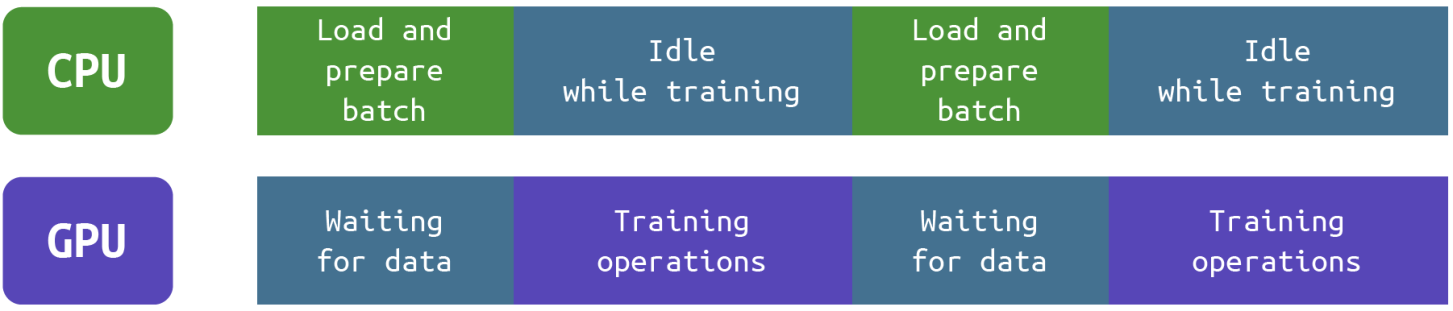
\includegraphics[width=\textwidth]{../images/GPU_CPU_Data_Training_2.pdf}}

\end{frame}

\begin{frame}[fragile]{Deep Learning with Data Parallelism}
\protect\hypertarget{deep-learning-with-data-parallelism-10}{}

\begin{itemize}
\tightlist
\item
  Data parallelism: proper data feeding for each worker

  \begin{itemize}
  \tightlist
  \item
    data pipelines: handled either by

    \begin{itemize}
    \tightlist
    \item
      internal TensorFlow (see tutorial) or PyTorch routines
    \item
      specialized libraries, e.g.~NVIDIA DALI, WebDataset
    \end{itemize}
  \end{itemize}
\end{itemize}

\begin{lstlisting}[language=Python]
# Example for TensorFlow dataset API
import tensorflow as tf

[...]

# Instantiate a dataset object
dataset = tf.data.Dataset.from_tensor_slices(files)

[...]

# Apply input preprocessing when required
dataset = dataset.map(decode, num_parallel_calls=tf.data.AUTOTUNE)
dataset = dataset.map(preprocess, num_parallel_calls=tf.data.AUTOTUNE)

# Randomize
dataset = dataset.shuffle(buffer_size)

# Create a batch and prepare next ones
dataset = dataset.batch(batch_size)
dataset = dataset.prefetch(tf.data.AUTOTUNE)

[...]
\end{lstlisting}

\end{frame}

\begin{frame}{Deep Learning with Data Parallelism}
\protect\hypertarget{deep-learning-with-data-parallelism-11}{}

\begin{itemize}
\tightlist
\item
  Data parallelism: proper data feeding for each worker

  \begin{itemize}
  \tightlist
  \item
    important not to let GPUs ``starve'' while training
  \item
    data handling via \textbf{data pipelines} routines
  \item
    use efficient \textbf{data containers}: HDF5, LMDB, TFRecords,
    WebDataset, \ldots{}
  \end{itemize}
\end{itemize}

\center{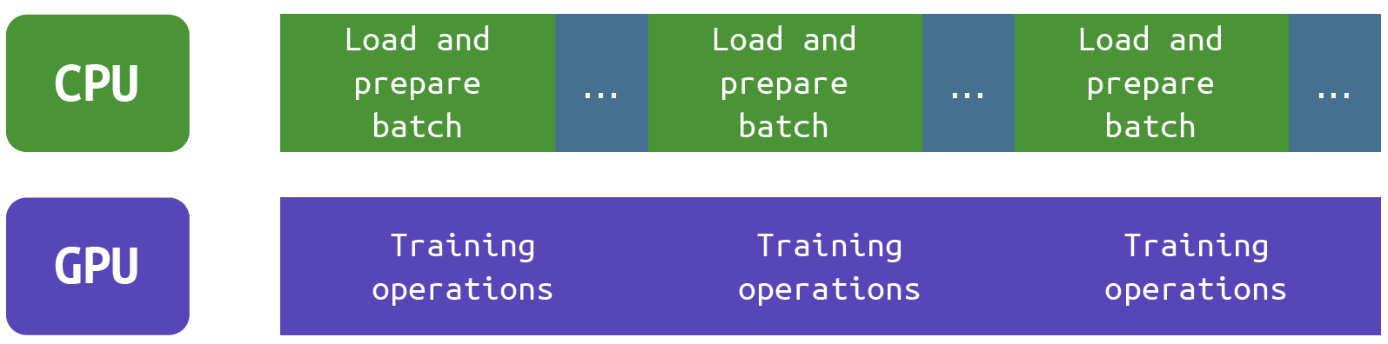
\includegraphics[width=0.9\textwidth]{../images/GPU_CPU_Data_Training_1.pdf}}

\end{frame}

\begin{frame}{Deep Learning with Data Parallelism}
\protect\hypertarget{deep-learning-with-data-parallelism-12}{}

\begin{itemize}
\tightlist
\item
  Data parallel distributed training requires:

  \begin{itemize}
  \tightlist
  \item
    proper data feeding for each worker: \emph{data pipelines,
    containers}
  \item
    setting up workers, one per each GPU (model clones)
  \item
    \textbf{sync of model clone weights} across workers: update step
    \(\mathbf{W}_{t+1} \leftarrow \mathbf{W}_t - \eta \nabla_\mathbf{W} \mathcal{L}_{\mathfrak{B}}\)

    \begin{itemize}
    \tightlist
    \item
      after each forward/backward pass on workers' mini-batches
    \item
      \(\nabla_\mathbf{W} \mathcal{L}_{\mathfrak{B}} = \dfrac{1}{K} {\displaystyle \sum_{j = 1}^{K} } \underbrace{\nabla_\mathbf{W} \dfrac{1}{n} {\displaystyle \sum_{X_i \in B_j} \mathcal{L}_i}}_{\text{on worker } j}\)
    \end{itemize}
  \end{itemize}
\end{itemize}

\vspace*{-1.5cm}
\center{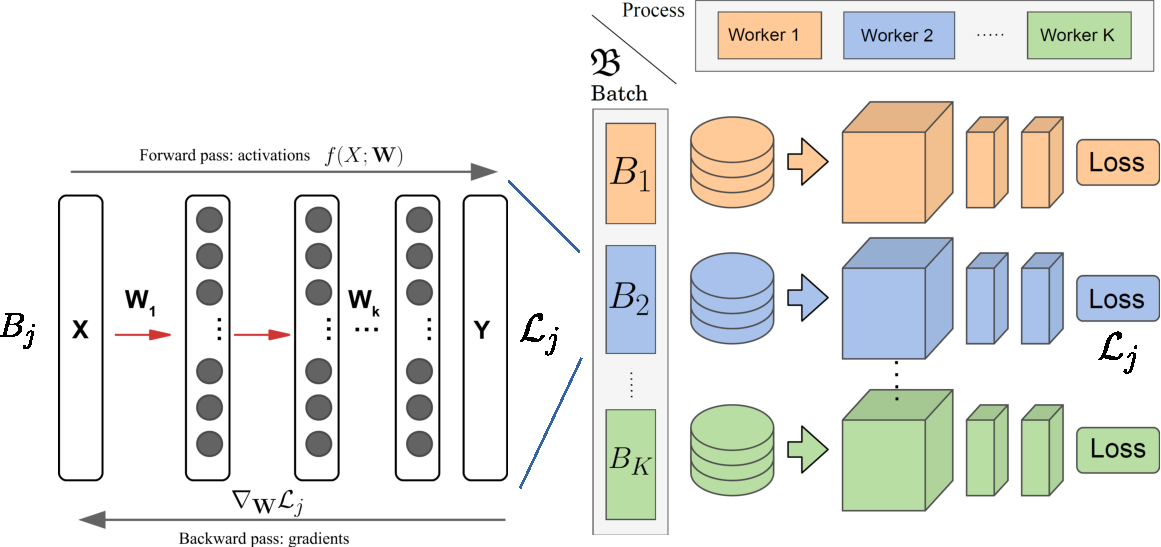
\includegraphics[width=0.8\textwidth]{../images/Forward_Backward_Data_Parallel_Workers_Batches.pdf}}

\end{frame}

\begin{frame}{Deep Learning with Data Parallelism}
\protect\hypertarget{deep-learning-with-data-parallelism-13}{}

\begin{itemize}
\tightlist
\item
  Data parallel distributed training requires:

  \begin{itemize}
  \tightlist
  \item
    proper data feeding for each worker: \emph{data pipelines,
    containers}
  \item
    \textbf{sync of model clone weights} across workers: handle
    communication between nodes

    \begin{itemize}
    \tightlist
    \item
      for large \(K\) and large model size -- high bandwidth required!
      Enter stage \textbf{InfiniBand} -- HPC
    \item
      efficient internode communication while training on GPUs! Enter
      stage \textbf{Horovod}, \textbf{PyTorch DDP}, \ldots{}
    \end{itemize}
  \end{itemize}
\end{itemize}

\center{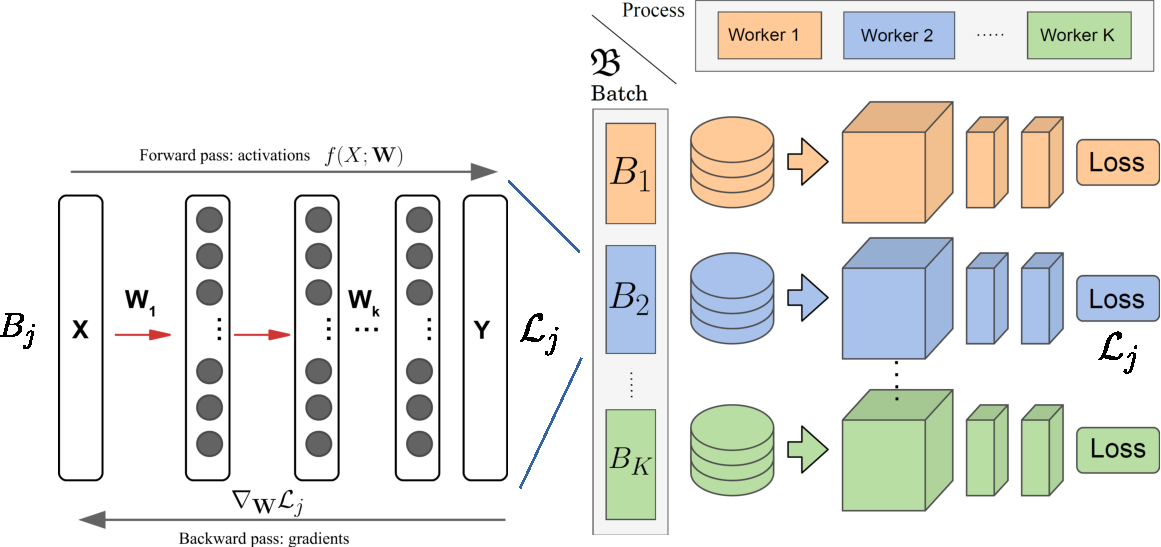
\includegraphics[width=0.8\textwidth]{../images/Forward_Backward_Data_Parallel_Workers_Batches.pdf}}

\end{frame}

\begin{frame}{Deep Learning with Data Parallelism: Horovod}
\protect\hypertarget{deep-learning-with-data-parallelism-horovod}{}

\begin{itemize}
\tightlist
\item
  Horovod: making data parallel distributed training easy

  \begin{itemize}
  \tightlist
  \item
    efficient worker communication during distributed training

    \begin{itemize}
    \tightlist
    \item
      synchronous, decentralized (\textbf{no} parameter servers,
      ring-AllReduce)
    \item
      additional mechanisms like Tensor Fusion
    \end{itemize}
  \item
    works seamlessly with job managers (Slurm)
  \item
    very easy code migration from a working single-node version
  \end{itemize}
\end{itemize}

\center{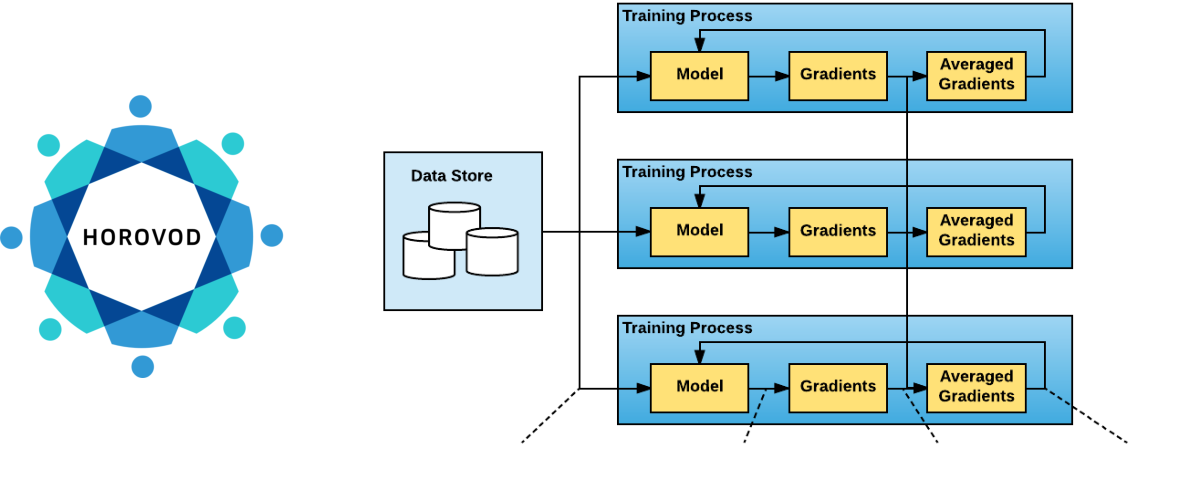
\includegraphics[width=0.8\textwidth]{../images/Horovod_Logo_Training_Combined.pdf}}

\vspace{-0.5cm}

\footnote<.->{\tiny Sergeev, A., Del Balso, M., 2017}

\end{frame}

\begin{frame}{Deep Learning with Data Parallelism: Horovod}
\protect\hypertarget{deep-learning-with-data-parallelism-horovod-1}{}

\begin{itemize}
\tightlist
\item
  Supports major libraries: TensorFlow, PyTorch, Apache MXNet
\item
  Worker communication during distributed training

  \begin{itemize}
  \tightlist
  \item
    NCCL: highly optimized GPU-GPU communication collective routines

    \begin{itemize}
    \tightlist
    \item
      same as in MPI: \texttt{Allreduce}, \texttt{Allgather},
      \texttt{Broadcast}
    \end{itemize}
  \item
    MPI: for CPU-CPU communication
  \item
    Simple scheme: 1 worker -- 1 MPI Process
  \item
    Process nomenclature as in MPI: \texttt{rank}, \texttt{world\_size}
  \item
    for local GPU assignment: \texttt{local\_rank}
  \end{itemize}
\end{itemize}

\center{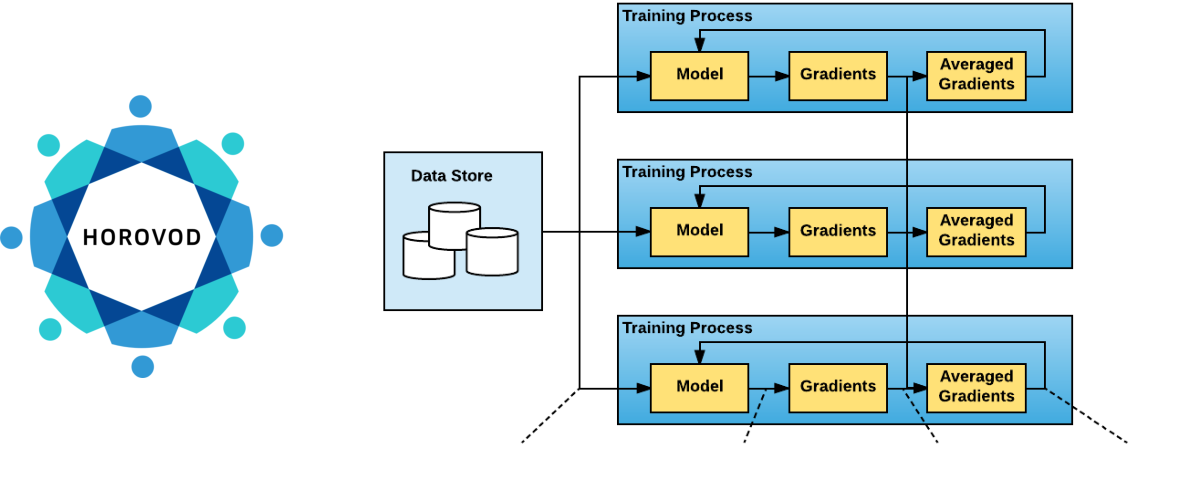
\includegraphics[width=0.8\textwidth]{../images/Horovod_Logo_Training_Combined.pdf}}

\end{frame}

\begin{frame}{Deep Learning with Data Parallelism: Horovod}
\protect\hypertarget{deep-learning-with-data-parallelism-horovod-2}{}

\begin{itemize}
\tightlist
\item
  Horovod: highly optimized library for data parallel distributed
  training

  \begin{itemize}
  \tightlist
  \item
    Name origin: ``horovod'' stands for east slavic (Ukraine, Russia,
    Bulgaria, Belarus, Poland, \ldots{}) circle dance form
  \end{itemize}
\end{itemize}

\center{
\includegraphics[width=0.4\textwidth]{../images/Horovod_Logo.pdf}}

\end{frame}

\begin{frame}{Distributed Training with Horovod}
\protect\hypertarget{distributed-training-with-horovod}{}

\begin{itemize}
\tightlist
\item
  Training model with a large effective mini-batch size:

  \begin{itemize}
  \tightlist
  \item
    \(\mathfrak{B} = \bigcup_{i \le K} B_i\),
    \(B_i \cap B_j = \emptyset,\ \forall i,j \in K\);
    \(\vert \mathfrak{B} \vert = K \cdot \vert B_{\text{ref}} \vert\)
  \item
    \(B_{\text{ref}}\) is reference batch size for single worker
  \end{itemize}
\end{itemize}

\center{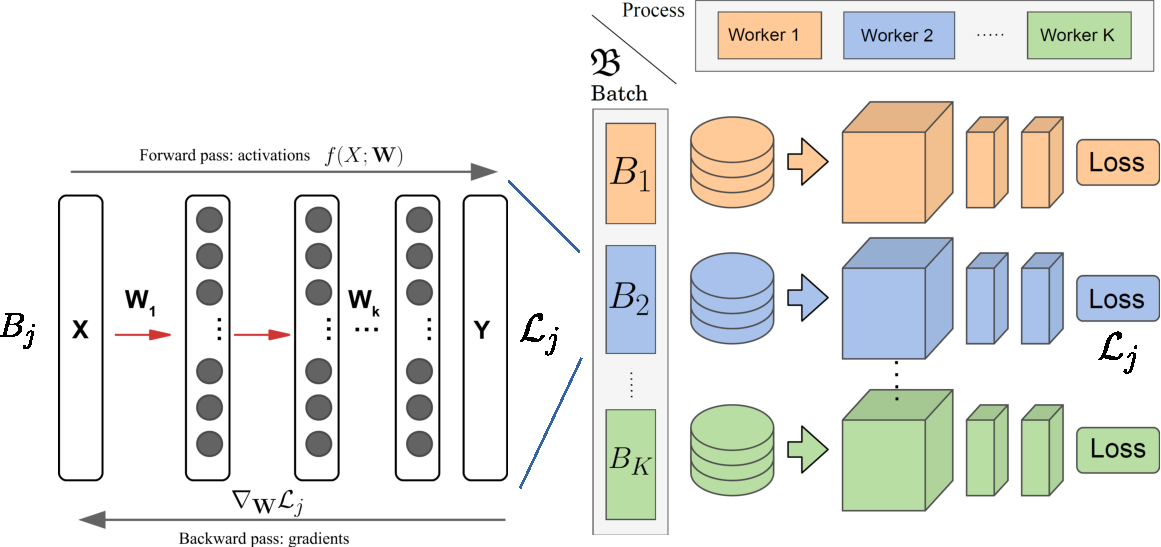
\includegraphics[width=0.8\textwidth]{../images/Forward_Backward_Data_Parallel_Workers_Batches.pdf}}

\end{frame}

\begin{frame}[fragile]{Distributed Training with Horovod}
\protect\hypertarget{distributed-training-with-horovod-1}{}

\begin{itemize}
\tightlist
\item
  Training loop: \(K\) workers, one per each GPU
\end{itemize}

\begin{lstlisting}
init: sync weights of all K workers
for e in epochs:
  shard data subsets D_j to workers j
  for B in batches:
    each worker j gets its own B_j (local compute)
    each worker j computes its own dL_j (local compute)
    Allreduce: compute dL_B, average gradients (communication)
    Update using dL_B for all K workers (local compute)
\end{lstlisting}

\center{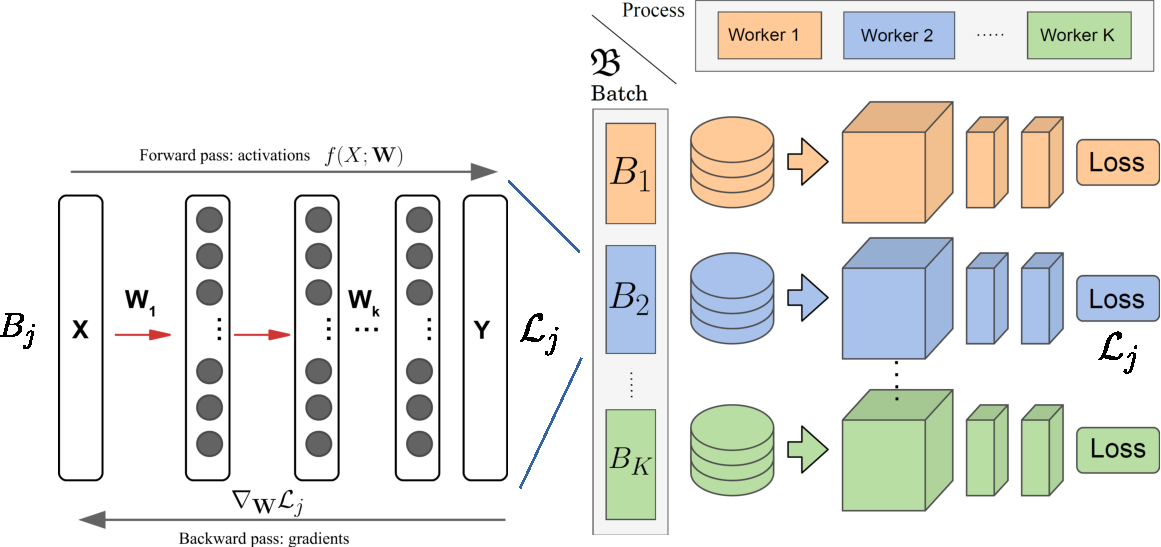
\includegraphics[width=0.6\textwidth]{../images/Forward_Backward_Data_Parallel_Workers_Batches.pdf}}

\end{frame}

\begin{frame}[fragile]{Distributed Training with Horovod}
\protect\hypertarget{distributed-training-with-horovod-2}{}

\begin{itemize}
\tightlist
\item
  User friendly code migration, simple wrapping of existing code

  \begin{itemize}
  \tightlist
  \item
    major libraries supported: TensorFlow, PyTorch, MXNet, \ldots{}
  \end{itemize}

  \begin{columns}[T]
  \begin{column}{0.5\textwidth}
\begin{lstlisting}[language=Python]
import tensorflow as tf
import horovod.tensorflow.keras as hvd

# Initialize Horovod
hvd.init()

[...]

# Wrap optimizer in Horovod's DistributedOptimizer
opt = hvd.DistributedOptimizer(opt)

[...]
\end{lstlisting}
  \end{column}

  \begin{column}{0.5\textwidth}
\begin{lstlisting}[language=Python]
import torch
import horovod.torch as hvd

# Initialize Horovod
hvd.init()

[...]

# Wrap optimizer in Horovod's DistributedOptimizer
opt = hvd.DistributedOptimizer(opt)

[...]
\end{lstlisting}
  \end{column}
  \end{columns}
\end{itemize}

\end{frame}

\begin{frame}{Distributed Training with Horovod}
\protect\hypertarget{distributed-training-with-horovod-3}{}

\begin{itemize}
\tightlist
\item
  Handled by dataset pipeline (Horovod independent): data sharding
\end{itemize}

\center{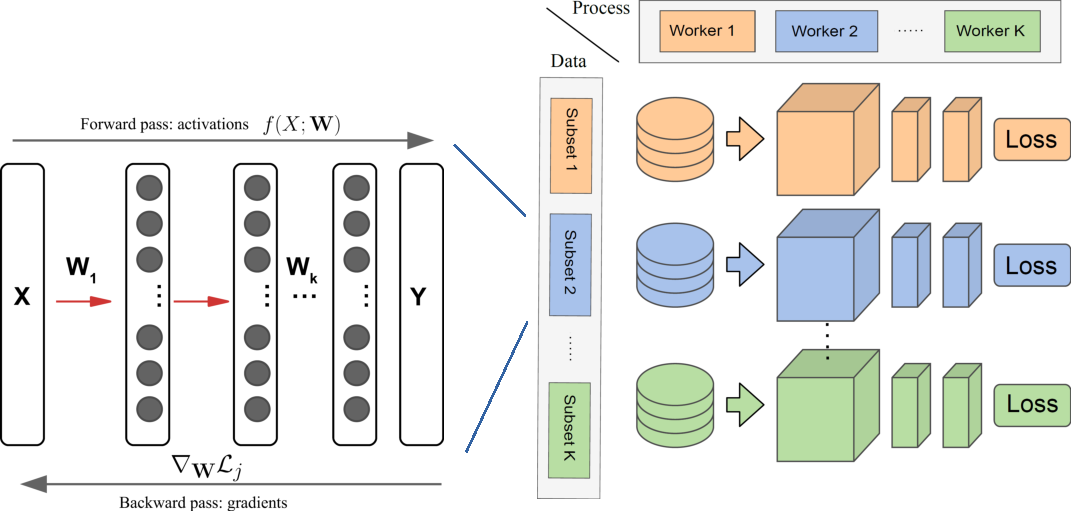
\includegraphics[width=\textwidth]{../images/Data_Parallel_Model_Workers_Processes_Data_Subsets.pdf}}

\end{frame}

\begin{frame}[fragile]{Distributed Training with Horovod}
\protect\hypertarget{distributed-training-with-horovod-4}{}

\begin{itemize}
\tightlist
\item
  Handled by dataset pipeline (Horovod independent): data sharding
\end{itemize}

\begin{lstlisting}[language=Python]
# Example for TensorFlow dataset API
import tensorflow as tf
import horovod.tensorflow.keras as hvd

[...]

hvd.init()

# Instantiate a dataset object
dataset = tf.data.Dataset.from_tensor_slices(files)

[...]

# Get a disjoint data subset for the worker
dataset = dataset.shard(hvd.size(), hvd.rank())

[...]

# Randomize
dataset = dataset.shuffle(buffer_size)

# Create worker's mini-batch and prepare next ones
dataset = dataset.batch(batch_size)
dataset = dataset.prefetch(tf.data.AUTOTUNE)

[...]
\end{lstlisting}

\end{frame}

\begin{frame}[fragile]{Distributed Training with Horovod}
\protect\hypertarget{distributed-training-with-horovod-5}{}

\begin{itemize}
\tightlist
\item
  Create a Slurm job script for the code wrapped with Horovod

  \begin{itemize}
  \tightlist
  \item
    \(K\) Horovod workers correspond to \(K\) tasks in total, 1 MPI
    process each
  \item
    \(K = \text{nodes} \cdot \text{tasks-per-node}\) =
    \(\text{nodes} \cdot \text{gpus-per-node}\)
  \end{itemize}
\end{itemize}

\begin{lstlisting}[language=bash]
#!/bin/bash

#SBATCH --account=training2306
#SBATCH --nodes=2
#SBATCH --ntasks-per-node=4
#SBATCH --cpus-per-task=20
#SBATCH --time=00:20:00
#SBATCH --gres=gpu:4
#SBATCH --partition=dc-gpu

srun python train_model.py
\end{lstlisting}

\center{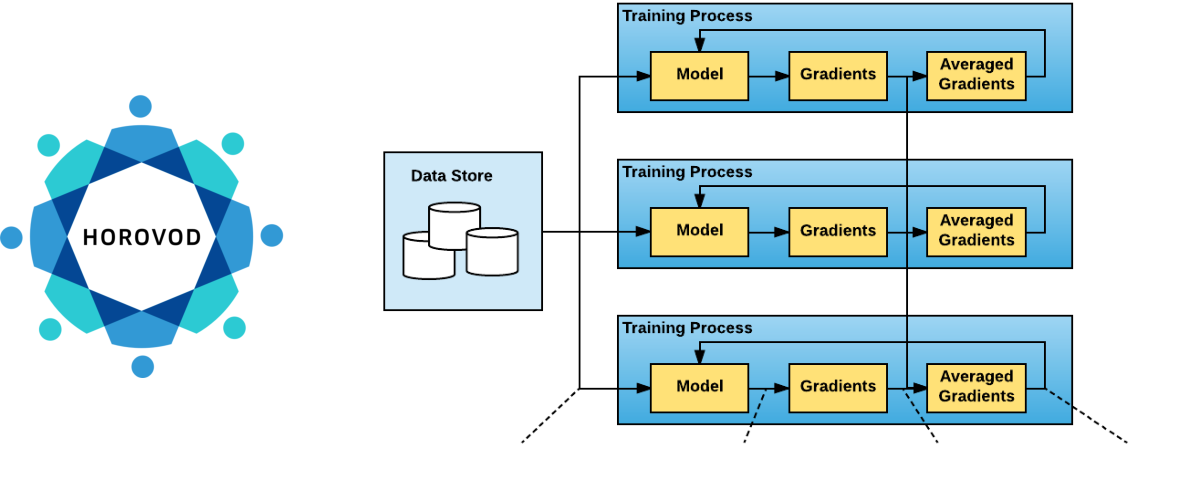
\includegraphics[width=0.6\textwidth]{../images/Horovod_Logo_Training_Combined.pdf}}

\end{frame}

\begin{frame}{Distributed Training with Horovod}
\protect\hypertarget{distributed-training-with-horovod-6}{}

\begin{block}{Basics to parallelize your model}

\begin{itemize}
\tightlist
\item
  Use Horovod to wrap existing model code
\item
  Use data containers and pipelines to provide data to workers
  efficiently
\item
  Create a Slurm job script to submit the wrapped code
\end{itemize}

\end{block}

\center{
\includegraphics[width=0.3\textwidth]{../images/Horovod_Logo.pdf}}

\end{frame}

\begin{frame}{Data Parallel Distributed Training}
\protect\hypertarget{data-parallel-distributed-training}{}

\begin{block}{Summary}

\begin{itemize}
\tightlist
\item
  Opportunity to efficiently speed up training on large data
\item
  Requires \(K\) GPUs, the larger \(K\), the better
\item
  Training with a larger effective batch size
  \(\vert \mathfrak{B} \vert = K \vert B_{\text{ref}} \vert\)
\item
  Data pipelines, high bandwidth network (InfiniBand) pave the way
\item
  Horovod, PyTorch DDP, TensorFlow DistributedStrategies
\item
  Additional measures to stabilize training -- upcoming lectures
\end{itemize}

\end{block}

\center{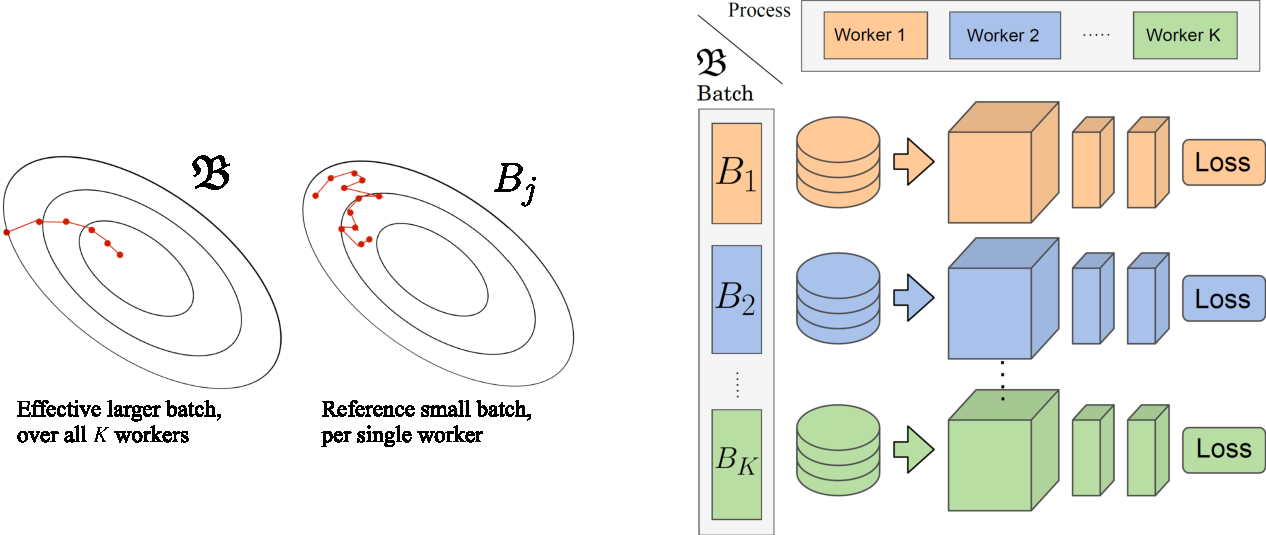
\includegraphics[width=0.65\textwidth]{../images/Large_Small_Reference_Batch_Data_Parallel_Model_Workers_Processes.pdf}}

\end{frame}
